d\documentclass[a4paper, oneside]{discothesis}

\usepackage[utf8]{inputenc}
\usepackage[T1]{fontenc}
\setlength{\parindent}{0pt}
\setlength{\parskip}{1em}
\usepackage{subcaption}
\usepackage{graphicx}
\usepackage{longtable}
\usepackage{placeins}


%%%%%%%%%%%%%%%%%%%%%%%%%%%%%%%%%%%%%%%%%%%%%%%%%%%%%%%%%%%%%%%%%%%%%%%%%%%%%%%%%%%%%%%%%%%%%%%%%
% DOCUMENT METADATA

\thesistype{Master's Thesis} % Master's Thesis, Bachelor's Thesis, Semester Thesis, Group Project
\title{Heritability of methylation patterns and their components}

\author{Brynja Sigurpalsdottir}
\email{brynjas@student.ethz.ch}

\institute{Computational Biology Group \\[2pt]
Department of Biosystems and Engineering \\[2pt]
ETH Zürich}

% Optionally, you can put in your own logo here
\logo{
\includegraphics[width=0.6\columnwidth]{figures/decode.png}}

%\supervisors{Supervisor 1, Supervisor 2\\[2pt] Prof.\ Dr.\ Roger Wattenhofer}

% Optionally, keywords and categories of the work can be shown (on the Abstract page)
%\keywords{Keywords go here.}
%\categories{ACM categories go here.}

\date{\today}

%%%%%%%%%%%%%%%%%%%%%%%%%%%%%%%%%%%%%%%%%%%%%%%%%%%%%%%%%%%%%%%%%%%%%%%%%%%%%%%%%%%%%%%%%%%%%%%%%

\begin{document}

\frontmatter % do not remove this line
\maketitle

\cleardoublepage

\begin{acknowledgements}
	I thank ..
\end{acknowledgements}

\begin{abstract}
    asdf
\end{abstract}

\tableofcontents

\mainmatter % do not remove this line


\chapter{Introduction}
% Byrjá á genome og genetic variations
    % Færa yfir í að ekki sé hægt að útskýra allar breytingar og sjúkdóma og því sé verið að færa í aukana að sequenca methylation status (epimutations)
    % Einn svoleiðis sjúkdómur er Kabuki syndrome - Búið að finna einhver gen en nú er talið að methylation munstrið spili enn mikilvægara hlutverk.

\section{Epimutations}
The completion of the Human Genome Project, has provided us with a nearly complete list of genes needed to produce a human. However, of equal importance is a second system that cells use to determine when and where a particular gene will be expressed during development. This system is overlaid on DNA in the form of epigenetic marks that are heritable during cell division but do not alter the DNA sequence \cite{robertson2005dna}. 

As with genes, these epigenetic marks can be mutated causing the genomic locus to deviate significiantly from the normal state. Those epimutations can be classified into two main types: primary epimutations that are thought to represent stochastic errors in the establishment or maintenance of an epigenetic state, while secondary epimutations are downstream events related to an underlying change in DNA sequence \cite{horsthemke2006epimutations}. The most common epigenetic modification of DNA (epimutation) in mammals is a methylation of the C5 position of cytosine in CpG dinucleotides, referred to as 5mC methylation. 

With recent dramatic advances in genomic technologies, genome-wide surveys of cohorts of patients with certain disorders or diseases for point mutations and structural variations have greatly advanced the understanding of their genetic etiologies. However, even after whole-genome-sequencing (WGS), no causative mutation can be identified in many such cases \cite{barbosa2018identification}. % laga citation

\section{Outline}
The goal of this thesis is to define the methylation signature of Kabuki syndrome using Oxford nanopore methylation data and determine the heritability of the methylation pattern.
\chapter{Background}

%%%%%%%%%%%%%%%%%%%%%%%%%%%%%%%%%%%%%%%%%%%%%%%%%
%%%%%%%%%%%%%%%%%%%%%%%%%%%%%%%%%%%%%%%%%%%%%%%%%
%%%%%%%%%%%%%%%%%%%%%%%%%%%%%%%%%%%%%%%%%%%%%%%%%
\section{Whole genome sequencing methods}
\label{sec:background:WGS}
Whole genome sequencing (WGS) is the process of determining the complete DNA sequence of an organism's genome at a single time. Capillary sequencing was the first approach to successfully sequence a nearly full human genome but since then technological developments have been crucial in enabling current population-scale human genome sequencing endeavours in research. By now, capillary sequencing has been progressively displaced by high-throughput, "next-generation" or "second-generation" sequencing technologies such as Illumina dye sequencing. Next generation sequencing is popular due to its massive parallelism, low-cost and deep coverage. Despite such advances, short-read lengths restrict the insight that can be derived from sequencing of an individual genome by limiting the resolution of repetitive or heterozygous regions, complex structural variation and haplotype phase. As a result, short-read sequencing is excellent for producing high quality, deep coverage of small to large genomes while important biological sequences such as genes or promoter regions are often highly fragmented \cite{alkan2011limitations}. 

Even though Illumina short-read sequencing is currently the most commonly used technique for human genome sequencing, so called "third generation sequencing" or long-read technologies have been rising in popularity. Third generation sequencing technologies get around the fundamental limitations of short-read sequencing for genome inference by providing more information per sequencing observation. In addition to increasingly being used within reference guided methods, long read technologies can generate highly contiguous \textit{de novo}  genome assemblies \cite{shafin2019efficient}. 

One of the "third-generation sequencing" methods that is particularly applicable to \textit{de novo} genome assembly because it can produce high yields of very long (100+ kilobase) reads is the Nanopore sequencing, commercialized by Oxford nanopore Technologies (ONT) \cite{jain2018nanopore}.

%%%%%%%%%%%%%%%%%%%%%%%%%%%%%%%%%%%%%%%%%%%%%%%%%
%%%%%%%%%%%%%%%%%%%%%%%%%%%%%%%%%%%%%%%%%%%%%%%%%

\subsection{Oxford Nanopore Technology}
\label{sec:background:ONT}



Nanopore sequencing uses eletrophoresis to transport an unknown sample through a nanoscaled orifice. Constant electric field is applied so an electric current can be observed in the system. The magnitude of the electric current density across a nanopore surface depends on the nanopore's dimension and the composition of the DNA or RNA that is occupying the nanopore. 

Nanopore sequencing technology is still being refined but it's portability and potential capability of generating long reads are of relevance to whole-genome sequencing applications. One challenge for this method was in refining the method to improve its resolution to be able to detect single bases. The low resolution is because the DNA strand moves rapidly at the rate of $1-5 \mu s$ per base through the nanopore. This makes recording difficult and prone to background noise, failing in obtaining single-nucleotide resolution. Oxford Nanopore employs a "kmer approach" to solve this problem, by analyzing more than one base at any one time so that stretches of DNA are subject to repeat interrogation as the strand moves through the nanopore one base at a time. %\cite{sequencing}

In Oxford Nanopore devices, an ionic current passes through nanopores, which are nano-scale holes, and the device measures the changes in current as biological molecules pass through the nanopore or near it. The information about the change in current can be used to identify that molecule. A strand of DNA is passed through the nanopore and the current is changed as the bases G, A, T and C pass through the pore in different combinations. % Skrifa meira!
%\cite{nanopore}

% Má hugsanlega sleppa
Currently the Oxford Nanopore offers three devices, MinION, GridION and PromethION. MinION can use up to 512 nanopore channels, GridION uses up to 5 MinION flow cells and PromethION uses up to 48 flow cells of 3000 nanopore channels each. deCODE started using PromethION in May 2018 and since then they have sequenced over 100 individuals. In the future PromethION is expected to be the leading device at deCODE and therefore I focused on the promethION data for this project.

\subsection{Targeted next generation sequencing}
\label{sec:background:NGS}
There are many genetic application that would benefit more by having sequence data from a large number of samples for specific genes rather than whole genomes. In these studies, researchers might have identified genes of interest and their goal is to sequence these genes from thousands of individuals. For this purpose, the most widely used method is targeted amplicon sequencing (TAS), which is a simple and cost effective method \cite{bybee2011targeted}.

TAS is a two step polymerase chain reaction (PCR) process that allows researchers to amplify a targeted gene region using traditional PCR, followed by an additional PCR step, where a known 10bp tag, or multiplexing identifier (MID), is attached to identify amplicons from different samples. This results in tagged amplicons that are ready to be sequenced using next generation platform, without extensive amplicon preparation steps or purchasing every possible combination of MID-locus specific primer \cite{bybee2011targeted}.

\section{DNA Methylation}
\label{sec:background:methylation}
In mammals, DNA methylation is an epigenetic mechanism involving the transfer of a methyl group on to one of the DNA bases, without changing the nucleotide sequence.
Methylation most commonly occurs at the 5-th carbon atom of the cytosine base within CpG dinucleotide and plays important role in many biological procedures such as regulating gene expression by recruiting proteins involved in gene repression or by inhibiting the binding of transcription factors to DNA. Increased methylation in the promoter region of a gene leads to reduced expression, whereas methylation in the transcribed region has a variable effect on gene expression \cite{das2004dna}. 

During development, the pattern of DNA methylation in the genome changes as a result of a dynamic process involving both de novo DNA methylation and demethylation. As a consequence, differentiated cells develop a stable and unique DNA methylation pattern that regulates tissue-specific gene transcription. 
Additionally it plays a pivotal role in embryonic development, cellular proliferation, differentiation and chromosome stability leading to development of human diseases. The importance of DNA methylation creates an urgent demand for effective methods with highly sensitivity and reliability to explore innovative diagnostic and therapeutic strategies \cite{li2011dna}.


%%%%%%%%%%%%%%%%%%%%%%%%%%%%%%%%%%%%%%%%%%%%%%%%%%%%%%%%%%%%%%%%%%%%%%%%%%%%%%%%%%%%%%%%%%%%%%%%%%
%https://academic.oup.com/bioinformatics/article/31/9/1466/200539
% https://www.ncbi.nlm.nih.gov/pmc/articles/PMC6128408/

\subsection{Abnormal methylation pattern and syndromes}
\label{sec:background:abnormal-met}
Mutations in the genes encoding the epigenetic protein machinery that read, write and erase post translational signals on DNA and histone proteins are implicated in a wide range of neurodevelopmental disorders such as Kabuki syndrome and Wiedemann-Steiner syndrome. Kabuki and Wiedemann-Steiner syndromes share various characteristics and such as the distinct facial features, short stature, abnormal hair growth etc.
%Mutation in those genes causes abnormal methylation pattern.


\subsubsection{Kabuki Syndrome}
\label{sec:background:Kabuki-syndrome}
Kabuki syndrome is a rare congenital disorder characterized by distinct facial features, postnatal growth retardation, mild to moderate intellectual disabilities, organ malfunction, endocrinological and hematological abnormalities. Two mutations have been identified to cause Kabuki Syndrome: heterozyguos mutation in lysine (K)-specific methyltransferase 2D (KMT2D) and mutation in lysine (K)-specific demethylase 6A (KDM6A). This has led to the definition of two subtypes of KS: KMT2D autosomal-dominant KS type 1 (KS1) and KDM6A-associated, X-linked-dominant KS type 2 (KS2). KS1 is the most common type, and has been identified in 56-75\% of Kabuki syndrome cases while only 5-8\% of cases are identified as KS2. The remaining 17-39\% of the cases do not have a known variant, causing the Kabuki syndrome. \cite{bogershausen2016mutation}

\subsubsection{Wiedemann-Steiner Syndrome}
\label{sec:background:Wiedemann-Steiner}
Wiedemann-Steiner syndrom (WSS) is a rare congenital malformation syndrome, characterized by hypertrichosis cubiti (hairy elbows), short stature, intellectual disability and distinctive facial features, such as long eyelashes, thick eyebrows, down slanted and vertically narrowed palpebral fissures, wide nasal bridge and broad nasal tip. \cite{miyake2016delineation} Jones et al (2012) identified de novo heterozygous mutation in KMT2A (lysine [K]-specific methyltransferase 2A) in WSS patients. KMT2A encodes a histone methyltransferase that plays an important role in early development and hematopoiesis.\cite{jones2012novo}


\subsection{Bivalent regions}
Bivalent regions are regions where the chromatin segments of DNA, bound to histone proteins, have both repressing and activating epigenetic regulators. Normally these regulators work in opposition to each other, either to enchance or silence the expression of genes, they normally interact with chromatime at different times. In bivalent regions however, both types of regulators are interacting with the same domain at the same time. 
%https://www.sciencedirect.com/science/article/pii/S095506741200052X?via%3Dihub
 
\section{DNA Methylation detection}
There are currently few methods used to profile methylation. The 'gold standard' method is bisulfate genomic sequencing, where the DNA has to be bisulfate treated before sequencing. Another promising method, used with ONT data, is Nanopolish which detects the methylation directly from the raw sequencing data.

\subsection{Bisulfate genomic sequencing}
\label{sec:background:Bisulfate}
The current 'gold standard' method used to profile methylation is called bisulfate genomic sequencing and is based on conversion of genomic DNA by using sodium bisulfate. It is based on the finding that the amination reactions of cytosine and 5mC proceed with different consequences after treatment of sodium bisulfate. Cytosines in single-stranded DNA will be converted into uracil residues and recognized as thymine in subsequent PCR amplification and sequencing. However 5mCs remain as cytosines allowing them to be distinguished from unmethylated cytosines.   bisulfate sequencing analysis can not only identify DNA methylation status along the DNA single strand, but also detect the DNA methylation patterns of DNA double strands since the converted DNA strands are no longer self-complementary and the amplification products can be measured individually \cite{frommer1992genomic} \cite{li2011dna}.

Bisulfate sequencing treatment results in extensive DNA fragmentation. Any breaks in the insert prevent downstream amplification and therefore high levels of input DNA is needed. This complicates the analysis as the epigenome is highly variable and results in a heterogeneous mixture of epigenic states. In addition short reads only reveal short-range patterns of methylation \cite{miura2012amplification}.

\subsubsection{Normalization with Limma}

\subsubsection{Detecting differentially methylated regions using Bumphunter method}
The bumphunting method for finding spatial intervals in which an estimated function (e.g. average difference between outcome groups) is different from 0 is referred to as bump hunting or peak detection. Bumphunter is a method developed to identify genomic regions associated with disease via genomic-scale microarray-based epigenomic data and epidemiological disease-related (covariate/exposure/phenotype) data.

They define the relationship between methylation, disease phenotype covariates and potential confounding due to batch effects via Equation \ref{eqn:bumphunter}

\begin{equation}
    \label{eqn:bumphunter}
    Y_{ij} = \mu(t_j) + \beta(t_j)X_i + \sum_{k=1}^p \gamma_k (t_j)Z_{i,k} + \sum_{l = 1}^q a_{l,j}W_{i,l} + \epsilon_{i,j}
\end{equation}

where $Y_{ij}$ is the epigenomic measurement (e.g. percentage of DNA methylation) at the j-th genomic locus for individual i, $t_j$ is the location on the genome of the j-th locus (i.e. chr 2, pos 42233500) and $\mu(t_j)$ is the population baseline level of the epigenomic measurement. $X_i$ represents the outcome of interest and $\beta(t_j)$ measures the association between the outcome of interest and the epigenomic measurement $Y_{ij}$ at location $t_j$. The $Zs$ denotes the potential measured confounders (e.g. sex, age, race) and $\gamma_k (t_j)$ represent the effects of confounder k at locus $t_j$, with each column of $Z$ representing a different confounder. $W$ represents potential unmeasured confounders or batch effects estimated via SVA and $a_{l,j}$ is the effect of unmeasured confounder $l$ on locus $t_j$. $e_{i,j}$ denotes the remaining variability such as measurement error and natural biological variability. 

Regions of biological interest (where methylation levels are associated with the outcome of interest) is provided as the contiguous intervals $R_n, n = 1,...,N$ where $\beta(t_j) \neq 0$ for all $t\in R_n$. $\beta(t)$ can be modeled as a smooth function of genomic position t and for most of the genome $\beta(t)=0$. Therefore $\beta(t)$ can be thought of as a straight horizontal line with N bumps. The goal is to find those bumps, i.e. detect the $R_ns$ with the following four steps: 

\begin{enumerate}
    \item estimate $\beta(t_j)$ for each $t_j$
    \item use these to estimate the smooth function $\beta(t)$
    \item Use this to estimate the regions $R_n$
    \item Use permutation test to assign statistical uncertainty to each estimated region \cite{jaffe2012bump}
\end{enumerate}

%%%%%%%%%%%%%%%%%%%%%%%%%%%%%%%%%%%%%%%%%%%%%%%%%
%%%%%%%%%%%%%%%%%%%%%%%%%%%%%%%%%%%%%%%%%%%%%%%%%
\subsection{Nanopolish}
\label{sec:background:nanopolish}
The electronic signal in nanopore is sensitive to modifications of the bases, such as methylations. Previous work has shown that by analysing the electronic current measured by nanopore sequencing device, 5-mC can be distinguished from cytosine. Nanopolish is a method to directly detect DNA modifications such as 5-mC, based on only the electrical readout of the ONT MinION instrument, without any chemical treatment \cite{simpson2017detecting}.

Nanopolish uses hidden Markov model (HMM) to analyze nanopore sequencing data. In short, HMM contains a set of emission distribution functions that model the probability of some observed data for each state of the model. For ONT sequencing data, the observations are segmented electrical current samples, referred to as event - where each event represent the current level measured over a time interval. The emission distribution functions model the event observation using Gaussian distribution with mean and s.d. depending on the particular short sequence, or k-mer which in this case is a 6-mer.

\subsubsection{The nanopolish hidden Markov model}
The hidden Markov model calculates the probability of observing a sequence of electric current events $e_1,...,e_n$ given a nucleotide sequence $S$. $S$ determines the structure of the model, the transition probabilities and emission distribution used in each state. Nanopolish has developed two different models, depending on what kind of nanopores are used to generate the data, R7.3 or R9. We only use data generated by R9 nanopores and therefore that is the only model we describe. For more information about the R7.3 model, see Supplementary Note in the article by Simpson \cite{simpson2017detecting}.

%The R7.3 model has a block of states for every k-mer of $S$ (6-mer) with each block containing a match state (indicating a particular event was observed from a particular k-mer), an extra state (indicating additional observations of events from a particular k-mer, reachable from the match state) and skip state (indicating no event observations for a k-mer). The transition probabilities are ...

The R9 model has a block of states for each k-mer of $S$. In each block there is a match and skip state to match an event to a k-mer and allow no observation from a k-mer, respectively. The match state has a self-transition to allow additional observations of events from a particular k-mer. There is also a bad state to account for the fact that some events have poorly estimated levels that do not match any expected state well. Finally there is a softclip state that allows events at the start and end of the event sequence to go unaligned, to account for uncertainty in the end points of the event sequence. The skip probabilities are calculated from the k-mer sequence and the transition probabilities are set to constant values. Likelihood of a sequence $S$, defined as the probability of observing the sequence of events given the hidden Markov model parameterized by $S$ is given with Equation \ref{eqn:loglik_hmm}.

\begin{equation}
    \label{eqn:loglik_hmm}
    \mathcal{L}(S|e_1,...,e_n,\Theta_v) = P(e_1,...,e_n | S,\Theta_v)
\end{equation}

Where $\Theta_v$ is the complete set of model parameters and $v$ is the pore version used to measure the events (R7.3 or R9).

\subsubsection{The emission distributions}

The ONT R7.3 basecaller (Metrichor) is followed by modeling the probability of observing an event $e_i$ given that the true sequence in the pore is k-mer $k$ using a Gaussian distribution:

\begin{equation}
    \label{eqn:emission_distribution}
    P(e_i|k,\Theta_v) = \mathcal{N}(a+b\mu_k + ct_i, (d\sigma_k)^2)
\end{equation}

where $e_i$ is the measured current level for event $i$, $t_i$ is the time at which event $i$ is observed, $k$ is the k-mer, $\mu_k$ is the current level for k-mer k, $\sigma_k$ is the standard deviation of the current level for k-mer E$k$, a is the shift parameter, b is the scale parameter, c is the drift parameter and d is the var parameter. Parameters a,b,c and d are used to capture read-specific deviations from the base model $\mathcal{N}(\mu_k, \sigma_k^2)$. For R9 data, c = 0 and a linear least square problem is solved to calculate a, b, d using the event labels provided by the R9 Metrichor basecaller.
Equation \ref{eqn:emission_distribution} is the emission distribution for the match states of the HMM where $k$ is the
k-mer corresponding to the state. The skip state does not emit observations. The R9 bad state emits any event with probability 1. The softclip state has a log-scaled emission probability of -3.0 independent of the event observation. 

For each read a set of emission distributions is selected from one of the following models: template, complement.pop1 and complement.pop2, based on the inferred physical properties of the DNA. The template model is always selected for the first sequencing strand and if a hairpin is detected, one of the two complement models is selected for the second strand. We select the complement model that provides the best solution when solving the linear least squares problem to fit a,b and d. 

\subsubsection{Expanding the alphabet}
Since the goal is to calculate whether a particular reference base is methylated, the provided ONT model need to be expanded to include k-mers that contain methylated bases. To handle methylation, the alphabet is expected to include a new symbol M representing 5-methylcytosine $\Sigma_{CpG} = \{ A,C,G,T,M\}$. This increases the number of emission distributions from $4^6=4096$ to $5^6=15625$. However, most of these k-mers are invalid since we are only interested in measuring 5mC in CpG context (i.e. AMTAGA is invalid but GTAMGA and ACGTM are valid). This alphabet will be referred to as CpG alphabet. Later we will refer to the unmethylated version of a k-mer, where we change the M symbol to C.

\subsubsection{Training emission distributions}

Nanopolish uses MinION reads aligned to a reference genome to learn new parameters for the emission distributions for each k-mer for each of the three ONT strand models. 2D reads aligned in base-space are iterated over and realigned in event-space using Viterbi algorithm. During this procedure, a list of events aligned to each k-mer is collected for each ONT strand model. Event is used if it is not in the first or last 5 events of the alignment, if it was aligned to a match state of the HMM and if the duration is at least 2 milliseconds. After realigning all reads, new parameters are learned by fitting a Gaussian Mixture model. Prior to training k-mers over the CpG alphabet, all CG dinucleotides in the reference are changed to MG. The inital Gaussian parameters for unmethylated k-mers are taken from the ONT models. For the methylated k-mers the mean is set to the mean for the unmethylated version of the k-mer and the standard deviation is set to be one greater than the standard deviation for the unmethylated version. The standard deviation is increased to help align events in the case that there is a true difference in means between the methylated and unmethylated k-mer. 

To fit a Gaussian mixture model, let $E_x = (e_1,...,e_n)$ be the sequence of events aligned to k-mer x. First compute $E_x^\prime = (e_1^\prime,...,e_n^\prime)$ where $\e_i^\prime=\frac{e_i-a_i-c_i-t_i}{b_i}$ is a transformation of event i to account for the Metrichor shift, scale and drift parameters. In the absence of methylation, we would have $P(e_i^\prime) =\mathcal{N} (\mu_x,((d_i/b_i)\sigma_x)^2)$. To account for incomplete enzymatic methylation in the training data, we fit a two component Gaussian mixture model to $E_x^\prime$ when x contains a methylated loss (k-mer contains M):

\begin{equation}
    \label{eqn:GaussianMixture}
    P(e_i^\prime) = w_1 \mathcal{N}(\mu_1, ((d_i/b_i)\sigma_1)^2) + w_2 \mathcal{N}(\mu_2, ((d_i/b_i)\sigma_2)^2)
\end{equation}

where $w_1, w_2$ are mixture weights representing the proportion of events that originate from methylated and unmethylated versions of x $(w_1+w_2=1)$. Parameters $w_j, \mu_j, \sigma_j$ are then fitted using ten iterations of the expectation-maximization algorithm (EM). Let $Z_i$ be a random variable indicating the component observation that i comes from and $x_j$ be the k-mer for the j-th component of the mixture. First the responsibility of omponent j for observation i is calculated:

\begin{equation}
    \label{eqn:responsibility}
    r_{i,j} = \frac{P(e_i|Z_i=j, x_j,\Theta)w_j}{\sum_{j = 1}^2 P(e_i | Z_i = j, x_j, \Theta}
\end{equation}

Then the weights and Gaussian parameters are updated:

\begin{equation}
w_j^\prime = \frac{\sum_{i = 1}^n r_{i,j}}{n}
\end{equation}

\begin{equation}
\label{eqn:mu_prime}
\mu_j^\prime = \frac{\sum_{i = 1}^n r_{i,j}e^\prime_i}{\sum_{i = 1}^n r_{i,j}}
\end{equation}

\begin{equation}
\label{eqn:sigma_prime}
\sigma_j^\prime = \frac{\sum_{i = 1}^n r_{i,j}((e^\prime_i-\mu_j^\prime)\frac{b_i}{d_i})^2}{\sum_{i = 1}^n r_{i,j}}
\end{equation}

When training k-mers with a methylation site, $w_1$ was initialized as 0.95 and the parameters $\mu_1^\prime, \sigma_1^\prime$ are used from the final iteration. When training k-mers that do not contain methylation sites a Gausssian distribution is fitted using Equation similar to Equations \ref{eqn:mu_prime}-\ref{eqn:sigma_prime} \cite{simpson2017detecting}.

We use both methylated regions and unmethylated regions for training and train the data over both nucleotide and CpG alphabet, generating four combinations of data type/alphabet for each pore type. Not all k-mers over the CpG alphabet can be trained, such as mixture of methylation sites (i.e. ACGMGT).

\subsubsection{Classifying CpG sites}
The substring of the reference genome that are tested for methylation is reffered to as $S_R$ and it is constructed such that it contains at least one, and possibly multiple $CG$ nucleotides plus flanking sequence that does not contain a $CG$. $CGs$ within $S_R$ is referred to as a group of sites. Sites are grouped together as the measured event current levels does not correspond to a single base rather than a k-mer, therefore closely-separated $CGs$ must be tested for methylation together. When testing for methylation it is assumed that all sites in the group have the same methylation status. The methylated version of $S_R$ is referred to as $S_M$. First the basecalled nanopore reads are aligned to a reference genome and then the alignments are used to find and group the $CG$ sites that are covered by a read. Group is called methylated or unmethylated using log likelihood ratios.

For each extracted and aligned read with mapping quality higher than or equal to 20, we iterate over the aligned segment of the reference genome and extract the locations of the CG dinucleotides. The list of covered $CG$ sites is partitioned into groups that are separated by at least 10bp and each group is tested for methylation independently. $c_s$ and $c_e$ are the position of the first and last $CG$ in the current group, then we extract the reference subsstring $S_R$ along with 10bp of flanking sequence: $S_R = reference[c_s-10 : c_e+10]$ and we also extract from the aligned nanopore reads the template and complete events aligned within the reference range $[c_s-10,...,c_e+10]$. The log likelihood ratio between $S_M$ and $S_R$ is then calculated using Equation \ref{eqn:loglik}.

\begin{equation}
\label{eqn:loglik}
    LogLikRatio(S_M) = \sum_{j=1}^2 log(\mathds{L}(S_M | e_{j,1},...,e_{j,n_j})-log(\mathds{L}(S_R | e_{j,1},...,e_{j,n_j})
\end{equation}

In some analyses there is a binary methylated or unmethylated classification of groups of $CG$ sites rather than working directly with the log likelihood ratio. Then a threshold $t$ is set on how extreme the log likelihood ratio must be to make a call. For a group consisting of $n$ $CG$ sites, the classification is only made if $|LogLikRatio(S_M)> nt|$ otherwise the group is ignored.


\subsubsection{Output example}
An example of a output from Nanopolish can be seen in Table \ref{table:nanopolish}.
\begin {table}[h]
    \caption{Example of Output from Nanopolish}
    \begin{center}
        \resizebox{\textwidth}{!}{\begin{tabular}{c c c c c c c c c c c} 
            \hline
            \textbf{chr} & \textbf{start} & \textbf{end} & \textbf{strand} & \textbf{read} & \textbf{loglik-ratio} & \textbf{loglik-met} & \textbf{loglik-unmet} & \textbf{num$\_$strands} & \textbf{num$\_$motifs} & \textbf{seq}\\
             \hline
             \hline
            chr1 & 10468 & 10470 & + & read1 & 1.26 & -132.54 & -133.8 & 1 & 2  & ACGT \\
            chr1 & 10468 & 10470 & + & read2 & 1.02 & -184.22 & -185.76 & 1 & 2  & ACGT \\
            chr1 & 10468 & 10470 & + & read3 & 1.40 & -359.23 & -361.45 & 1 & 2  & ACGT \\
            chr1 & 10468 & 10470 & + & read4 & 3.73 & -202.67 & -206.59 & 1 & 2  & ACGT \\
            chr1 & 10468 & 10470 & + & read5 & 1.54 & -214.79 & -2016.48 & 1 & 2  & ACGT \\
            \multicolumn{11}{c}{$\vdots$} \\
             \hline
        \end{tabular}}
    \label{table:nanopolish}
    \end{center}
\end{table}

\subsubsection{Methyl loglik}
As an addition to Nanopolish, we have a script that sums up all reads per position and returns the results per position. Additionally, the script returns some desirable statistics that help check how well nanopolish is performing. The script is written in GOR, which is an internal tool (See section...)%!!!!!!

Columns and their description can be seen in Table \ref{table:loglik} % MOVE TO APPENDIX? EXPLAIN THE MAIN COLS HERE

\begin {longtable}[h]{l p {8.5cm}}
    \caption{Explanation of the output from the methyl-loglik script}
    \label{table:loglik}
    \centering
        \hline
        \textbf{Column name} & \textbf{Description} \\
        \hline
        \hline
        \textbf{Chrom} & Chromosome \\[0.5ex]
        \textbf{start} & Start position of the read \\[0.5ex]
        \textbf{end} & End position of the read \\[0.5ex]
        \textbf{allCount} & Number of reads \\[0.5ex]
        \textbf{sum$\_$num$\_$motifs} & Total number of motifs (sum(num$\_$motifs)) \\[0.5ex]
         \textbf{sum$\_$plus$\_$met0} & Number of reads where the log likelihood ratio is larger than 0 on plus strand\\[0.5ex]
        \textbf{sum$\_$plus$\_$met} & Number of reads where the log likelihood ratio is larger than 1.921 on plus strand\\[0.5ex]
        \textbf{sum$\_$plus$\_$unmet0} & Number of reads where the log likelihood ratio is less than or equal to 0 on plus strand\\[0.5ex]
        \textbf{sum$\_$plus$\_$unmet} & Number of reads where the log likelihood ratio is less than -1.921 on plus strand\\[0.5ex]
        \textbf{sum$\_$plus$\_$cnt} & Total number of reads of the plus strand\\[0.5ex]
        \textbf{sum$\_$minus$\_$met} & Number of reads where the log likelihood ratio is less than -1.921 on minus strand\\[0.5ex]
        \textbf{sum$\_$minus$\_$unmet0} & Number of reads where the log likelihood ratio is less than or equal to 0 on minus strand\\[0.5ex]
        \textbf{sum$\_$minus$\_$unmet} & Number of reads where the log likelihood ratio is less than -1.921 on minus strand\\[0.5ex]
        \textbf{sum$\_$minus$\_$cnt} & Total number of reads of the minus strand\\[0.5ex]
        \textbf{sum$\_$met0} &  Total number of reads where the log likelihood ratio is larger than 0 (sum$\_$plus$\_$met0 + sum$\_$minus$\_$met0)\\[0.5ex]
        \textbf{sum$\_$met} &  Total number of reads where the log likelihood ratio is larger than 1.921 (sum$\_$plus$\_$met + sum$\_$minus$\_$met) \\[0.5ex]
        \textbf{sum$\_$unmet0} & Total number of reads where the log likelihood ratio is less than or equal to 0  (sum$\_$plus$\_$unmet0 + sum$\_$minus$\_$unmet0) \\[0.5ex]
        \textbf{sum$\_$unmet} & Total number of reads where the log likelihood ratio is less than -1.921 (sum$\_$plus$\_$unmet0 + sum$\_$minus$\_$unmet0) \\[0.5ex]
         \textbf{avg$\_$prob$\_$methylated} & Average probability that a position is methylated, $avg(exp(log\_lik\_ratio)/(a+log\_lik\_ratio))$\\[0.5ex]
         \textbf{avg$\_$plus$\_$prob$\_$methylated} & Average probability that a position on plus strand is methylated \\[0.5ex]
         \textbf{avg$\_$minus$\_$prob$\_$methylated} & Average probability that a aposition on minus strand is methylated \\[0.5ex]
         \pagebreak
         \textbf{ratio0} & Total number of reads where log likelihood ratio is larger than 0 out of all reads (sum$\_$met0/n$\_$total0)\\[0.5ex]
         \textbf{ratio} & Total number reads where log likelihood ratio is larger then 1.921 out of all reads (sum$\_$met/n$\_$total) \\[0.5ex]
         \textbf{ratio0$\_$plus} & Total number of reads on plus strand where log likelihood ratio is larger than 0 out of all reads on plus strand (sum$\_$plus$\_$met0/n$\_$plus0) \\[0.5ex]
         \textbf{ratio$\_$plus} & Total number of reads on plus strand where log likelihood ratio is larger than 1.921 out of all reads on plus strand that are either larger then 1.921 or less then -1.921 (sum$\_$plus$\_$met0/n$\_$plus)\\[0.5ex]
         \textbf{ratio0$\_$minus} &  Total number of reads on minus strand where log likelihood ratio is larger then 0 out of all reads on minus strand (sum$\_$minus$\_$met0/n$\_$minus0)\\[0.5ex]
         \textbf{ratio$\_$minus} & Total number of reads on minus strand where log likelihood ratio is larger than 1.921 out of all reads on minus strand that are either larger than 1.921 or less than -1.921 sum$\_$minus$\_$met/n$\_$minus\\[0.5ex]
         \hline
\end{longtable}



%%%%%%%%%%%%%%%%%%%%%%%%%%%%%%%%%%%%%%%%%%%%%%%%%
%%%%%%%%%%%%%%%%%%%%%%%%%%%%%%%%%%%%%%%%%%%%%%%%%
%%%%%%%%%%%%%%%%%%%%%%%%%%%%%%%%%%%%%%%%%%%%%%%%%

\section{Genome-wide association study (GWAS)}
\label{sec:background:GWAS}
Genome-wide association study (GWAS) is a study of a genome-wide set of genetic variants in many individuals to see if any variant is associated with a trait. Usually, GWAS focus on association between single-nucleotide polymorphisms (SNPs) and traits like human diseases. Researchers can use the information to develop better strategies to detect, treat and prevent the disease, once new genetic associations are identified. Such studies are particularly useful in finding genetic variations that contribute to common, complex diseases, such as asthma, diabetes, cancer, cardiovascular diseases and mental illnesses. 

%%%%%%%%%%%%%%%%%%%%%%%%%%%%%%%%%%%%%%%%%%%%%%%%%
%%%%%%%%%%%%%%%%%%%%%%%%%%%%%%%%%%%%%%%%%%%%%%%%%

\subsection{Polygenic risk score}
\label{sec:background:PRS}
The results from a genome-wide association study (GWAS) has revealed that much of the genetic basis for most complex traits comprises small effects of hundreds or even thousands of variants. These effects can be considered a genetic liability to disease risk. Polygenic risk score (PRS) is a sum of trait-associated alleles across many genetic loci, which is usually weighted by the effect sizes estimated from a GWAS. PRS can among others detect shared genetic aetiology among traits, can be used to infer the genetic architecture of a trait, for screening in clinical trials and act as a biomarker for a phenotype. 

Once quality control has been perfomed on the base and target data and the files have been formatted appropriately, the PRS can be calculated. GWAS is performed on finite samples drawn from particular subsets of the human population and so that the effect size estimates are some combination of true effect and stochastic variation. This causes the estimated effects to not generalize well to different population. Linkage disequlibrium (LD) can also complicate the aggregation of the data. Key factors in the developement of methods for calculating PRS are:
\begin{enumerate}
    \item adjusting GWAS estimated effect sizes via e.g. shrinkage and incorporation of their uncertainty
    \item the tailoring of PRS to target populations
    \item dealing with LD
\end{enumerate}

\subsubsection{Shrinkage of GWAS effect size estimates}
Given that a variants effects are estimated under uncertainty and not all variants influence the trait the use of unadjusted effect size estimates of all variants could generate poorly estimated PRS with high standard error. Therefore we can use either shrinkage of the effect estimates of all variants via standard or tailored statistical techniques such as LASSO/ridge regression, or use p-value selection threshold as inclusion criteria for variants into the score.

\subsubsection{Controlling for Linkage Disequilibrium}
The association tests in GWAS are typically performed one-variant-at-a-time, which combined with the strong correlation structure across the genome, makes identifying the independent genetic effects challenging. The power of GWAS can be increased by conditioning on the effects of multiple variants simultaneously. There are two main methods used: clumping or account for the linkage disequilibrium (LD). The first method involves clumping variants together so that the retained variants are largely independent of each other and thus their effects can be summed, assuming additivity. This method is usually used with p-value threshold. The second method is generally favoured in methods that implement traditional shrinkage methods.
%AÐALLEGA: https://www.biorxiv.org/content/biorxiv/early/2018/09/14/416545.full.pdf



\section{Theory}
% Subsection statistics?
\subsection{Independent two sample t-test}
The ratio of methylated samples detected by nanopolish was calculated for each position. Then the average and standard deviation within each population (Kabuki group and the control group) was calculated. Independent two-sample t-test was used to compare the means between the two populations. The two population variances are assumed be equal so Equation \ref{eqn:ttest} was used to calculate the t statistics. %using stats package in python?

\begin{equation}
\label{eqn:ttest}
    t = \frac{\bar{X}_1 - \bar{X}_2}{s_p\sqrt{\frac{1}{n_1}+ \frac{1}{n_2}}}
\end{equation}
where
\begin{equation}
\label{eqn:sdelta}
    s_p = \sqrt{\frac{(n_1-1)s_{X_1}^2+(n_2-1)s_{X_2}^2}{n_1+n_2-2}}
\end{equation}

$s_p$ is an estimator of the pooled standard deviation of the two samples. The pooled standard deviation is defined so that its square is an unbiased estimator of the common variance whether or not the population means are the same. $n_i-1$ is the number of degrees of freedom for each population and the total number of degrees of freedom is $n_1+n_2-2$. From the t value we can find the corresponding probability value (p-value) using python or R.

\subsection{Probability values (p-values)}
In hypothesis testing, p-value or probability value is the probability that, when the null hypothesis is true, the statistcal summary would be greater then or equal to the actual observed results. A p-value of 0.05 means that there is 5\% chance that you would get your observed results if the null hypothesis were true. In other words when we set p-value as 0.05 we are saying that there is 5\% chance that where we get a significant difference, in reality there is none (False positives). When dealing with large number of samples we could therefore get a lot of false positives. To deal with this problem most methods attempt to assign an adjusted p-value to each test or reduce the p-value treshold to a more reasonable value. Two widely used methods are Benjamini-Hochberg procedure and Bonferroni correction.

\subsubsection{Bonferroni correction}
When multiple hypothesis are tested, the chance of a rare event increases and therefore the likelihood of incorrectly rejecting a null hypothesis increases. Bonferroni correction recomposes for that increase by testing each hypothesis at a significance level calculated using Equation \ref{eqn:Bonferroni}, where $\alpha$ is the desired overall false positive level and N is the number of hypothesis.

\begin{equation}
    \label{eqn:Bonferroni}
        \alpha_{crit} = \frac{\alpha}{N}
\end{equation}


Bonferroni technique can be too conservative in the sense that while the number of false positives is reduced, the number of true discoveries is also reduced.


\subsubsection{Benjamini-Hochberg procedure}
Benjamini-Hochberg procedure is a procedure to determine the adjusted p-values (q-values) for each test. This method controls the number of false discoveries in those tests that result in significant results and is therefore less conservative then the Bonferroni correction and has greater ability to find truly significant results. The procedure is as follows:

\begin{enumerate}
    \item Sort the p-values in ascending order
    \item Assign ranks to the p-values, the smallest has a rank of 1, the second smallest a rank of 2, etc.
    \item Calculate the adjusted p values using Equation \ref{eqn:qval}, where i is the individuals p-values rank, N is the total number of tests and $\alpha$ is the False discovery rate.
        \begin{equation}
            \label{eqn:qval}
            q(i) = \frac{i\alpha}{N}
        \end{equation}
    \item Find the largest $p(i) < q(i)$, that is the Benjamini-Hochberg threshold.
\end{enumerate}


This method is often referred to The False Discovery rate procedeure. False discovery rate (FDR) is the rate of samples called significant are truly not. FDR of 5\% means that among all samples called significant, 5\% of those are truly not significant. 

\subsection{Fisher's Exact Test}
The Fisher exact test is a test of statistical significance that is used in the analysis of contingency tables, especially when sample size is small. Fisher's exact test examines the relationship between the two dimensions of the contingency table, shown in Table \ref{table:cont}. The null hypothesis is that these two classifications are not different and the significance of the deviation from a null hypothesis (p-value) is calculated.

\begin {table}
    \caption{Example of Contingency Table}
    \begin{center}
        \begin{tabular}{ c c c |c} 
            \hline
            &  \textbf{Outcome 1} & \textbf{Outcome 2} & \textbf{Total}\\
             \hline
             \hline
             \textbf{Group 1} & a & b & a+b \\ 
             \textbf{Group 2} & c & d & c+d \\
             \hline
             \textbf{Total} & a+c & b+d & N = a+b+c+d\\
             \hline
        \end{tabular}
    \label{table:cont}
    \end{center}
\end{table}

Fisher showed that the probability of obtaining any such set of values was given by the hypergeometric distribution. Equation \ref{eqn:hypergeom} gives the exact hypergeometric probability of observing this particular arrangement of the data on the null hypothesis. 

\begin{equation}
    \label{eqn:hypergeom}
    p = \frac{\binom{a+b}{a} \binom{c+d}{c}}{\binom{n}{a+c}} = \frac{\binom{a+b}{b} \binom{c+d}{d}}{\binom{n}{b+d}} = \frac{(a+b)\,!(c+d)\,!(a+c)\,!(b+d)\,!}{a\,!
    b\,!c\,!d\,!n\,!}
\end{equation}

\subsubsection{Log odds ratio}
Odds ratio (OR) quantifies the strength of the association between two events. It is defined as the ratio of the odds of Event 1 in the presence of Event 2 and the odds of Event 1 in the absence of Event 2 or the ratio of the odds of Event 2 in the presence of Event 1 and the odds of Event 2 in the absence of Event 1, due to symmetry. If OR = 1, the odds of one event are the same in either the presence or absence of another event. If OR > 1 then Event 1 and 2 are correlated in the sense that compared to the absence of Event 2, the presence of Event 2 raises the odds of Event 1 and symmetrically, the presence of Event 1 raises the odds of Event 2. If OR < 1, then Event 1 and 2 are negatively correlated and the presence of one event reduced the odds of the other event.

From the contingency table we can also calculate the Log odds ratio, given by Equation \ref{eqn:oddsratio}.

\begin{equation}
    \label{eqn:oddsratio}
    OR = \frac{a/b}{c/d} = \frac{a\cdot d}{c \cdot b} = \frac{a/b}{c/d}
\end{equation}



\subsection{Principal Component Analysis}
Principal component analysis or PCA is a widely used technique for applications such as dimensionality and noise reduction, feature extraction and data visualization. PCA can be defined as the orthogonal projection of the data onto a lower dimensional linear space such that the variance of the projected data is maximized. In other words, PCA searches for the linear combinations with the largest variances and divides them into Principal components (PCs). The first PC should capture the largest variance, the second PC should capture the second largest variance, etc. PCA is used in many applications such as exploratory data anlysis, making predictive models, visualize genetic distance and relatedness between populations. % Heimild pattern recognition bishop

In order to perfrom PCA a few steps have to be performed. Let $x_1,...,x_n$  be n vectors in $\mathbb{R}^2$ and $x_n$ is a Euclidean variable with dimension d. Assume we want to project the data into $d \times k$ dimension.

First the covariance matrix is computed using Equation \ref{eqn:cov}.

\begin{equation}
\label{eqn:cov}
\Sigma = cov(x, x^\intercal) = \frac{1}{n-1}\sum_{i = 1}^{n} (x_i - m)(x_i - m)^\intercal
\end{equation}
where m is the mean vector, given with Equation \ref{eqn:meanvec}:

\begin{equation}
\label{eqn:meanvec}
m = \frac{1}{n} \sum_{i = 1}^n x_i
\end{equation}

Next we need to factorize the covariance matrix to find the eigenvectors $v$ and corresponding eigenvalues$\lambda$ that fulfill Equation \ref{eqn:eign}.

\begin{equation}
\label{eqn:eign}
\Sigma v = \lambda v
\end{equation}

The eigenvectors are then sorted by decreasing eigenvalues and the k largest eigen vectors chosen (corresponding to the k largest eigenvalues). Those eigenvectors are equivalent to the principal components. The eigenvectors form a $d \times k$ dimensional eigenvector matrix $W$. Finally the samples are transformed onto the new subspace via Equation \ref{eqn:transform}.

\begin{equation}
\label{eqn:transform}
y = W^\intercal \times x
\end{equation}
where x is a $d\times1$ dimensional vector representing one sample and y is the transformed $k\times1$ dimensional sample in the new subspace.
% ATH FORMULUR!!

\subsubsection{Eigendecomposition}
One way to factorize the covariance matrix is to perform eigendecomposition, given by equation \ref{eqn:eigendecomp}.

\begin{equation}
    \label{eqn:eigendecomp}
    \Sigma = V \Lambda V^\intercal
\end{equation}

where V is the matrix containing the eigenvectors of $\Sigma$ along its columns and $\Lambda$ is a matrix containing the corresponding eigenvalues along the diagonal line and zeroess elsewhere. Only diagonalizable matrices can be factorized in this way.

\subsubsection{Singular Value Decomposition} % And relationship to PCA
Another closely related decomposition method that can be used for factorizing the matrices is the Singular value decomposition (SVD). It decomposes a matrix into the product of two unitary matrices ($U$ and $V$) and a rectangular diagonal matrix of the singular values $S$.

\begin{equation}
    \label{eqn:SVD}
    \underset{n\times m}{X} = \underset{n \times n}{U} \underset{n \times m}{S} \underset{m \times m}{V}
\end{equation}


PCA and SVD are closely related approaches and can both be applied to decompose any rectangular matrices. If we perform SVD on the covariance matrix $cov(x,x^\intercal)$ we get:
\begin{align*}
    \Sigma = Cov(x,x^\intercal) &= \frac{x^\intercal x}{n-1} \\
    &= \frac{VS U^\intercal U S V^\intercal}{n-1} \\
    &= V \frac{S^2}{n-1} V^\intercal \\
    &= V \frac{S^2}{n-1}V^{-1} \text{ (since V is unitary)} \\
\end{align*}

From the above derivation we can see that the result is in the same form as with eigendecomposition of $Cov(x, x^\intercal)$ and that the relationship between singular values  and eigenvalues from the previous chapter is given with equation \ref{eqn:singular}.

\begin{equation}
    \label{eqn:singular}
    \lambda_i = \frac{s_i^2}{n-1}
\end{equation}

SVD is therefore a generalization of eigendecomposition of a positive semidefinite normal matrix to any $m \times n$ matrix, where we no longer require the matrix to be diagonalizable.

\subsubsection{PCA for high-dimensional data} % PYSPARK OR RANDOM PCA
In some applications of PCA, the number of data points is much smaller then the dimensonality of the data space, for example when you have the methylation difference between ...

\subsection{Linear Regression}
Linear Regression is a linear approached used in statistics to model the relationship between a scalar response and explanatory variables or independent variables. Linear regression models the relationships using linear predictor functions whose unknown model paramters are estimated from the data. It has many practical uses but most applications fall into one of the following two categories:
\begin{itemize}
    \item Prediction: Linear regression can be used to fit a predictive model to an observed data set of values of the response and explanatory variables. If the additional values of the explanatory variables are collected without an accompanying response value, the fitted model can be used to make a prediction of the response.
    \item Variation explanation: Linear regression analysis can be applied to quantify the strength of the relationship between the response and explanatory variables, and in particular to determine whether some explanatory variables may have no linear relationship with the response at all, or to identify which subsets of explanatory variables may contain redundant information about the response.
\end{itemize}

These models are often fitted using the least squares approach.

\begin{equation}
y_i = \beta_0 1 + \beta_1 x_{i1} + ... + \beta_p x_{ip} + \epsilon_i = x_i^\intercal \beta + \epsilone_i, \text{ for } i = 1,...,n    
\end{equation}

\subsection{Support Vector Machine}


\section{Previous work}
To this day, two genes have been identified that cause KS, KMT2D and KDM6A. % references from HT greininni.

Majority of the Kabuki syndrome cases (55-80\%), are inherited as an autosomal dominant trait, caused by loss of function variants in lysine (K)-specific methyltransferase 2D (KMT2D) and in only a small fraction (4-12\%) of the cases the disorder shows X-linked dominant inheritance caused by loss of function variants in lysine (K)-specific dimethylase 6A (KDM6A). However, approximately 10-30\% of individuals with clinical features of KS will not be found to have mutations or deletions in either KMT2D or KDM6A, suggesting that other genes that encode proteins that couple with KMT2D or KDM6A or in related developmental pathways may account for this small subset of cases. % multiple references sjá greinar fra HT og review

\subsection{Sorbreira et al}
Sorbreira et al. \cite{sobreira2017patients} measured DNA methylation levels across the genome in 36 samples, 27 Kabuki and 9 control samples that matched on age, sex and ethnicity. DNA was isolated from peripheral blood cells in an identical manner in cases and controls. The probes were designed for targeted sequencing (TruSeq Custom Amplicon kit, Illumina) with the online Illumina DesignStudio software for all candidate genes including exon-intron boundaries. One library of 28 samples (27 individuals and 1 control) was sequenced in a single run on MiSeq sequencerr (Illumina, $2\times251$ bp paired end reads). %Alignment of NGS data to the human reference genome and variant calling were performed using software provided by Illumina. All variant calls were based on RefSeq transcript and NCBI human genome assembly build 37.
Genomic DNA was prepared, for each sample, in a total volume of 45 $\mu l$ using EZ DNA methylation kit and bisulfate treated as specified for use with Infinium Human Methylation 450 BeadChip arrays. Bisulfate treated DNA was processed on the Infinium HumanMethylation450 BeadChip, which measures DNA methylation levels at 485,512 loci across the genome. All samples were processed in parallel and case and control randomized across four 12-sample array BeadChips that were run in parallel to minimize potential confounding batch effects related to hybridization or laboratory conditions. The R-package Limma was used to identify differentially methylated positions (DMPs) and R package bumphunter was used to identify differentially methylated regions (DMRs). Both models were adjusted for sex, blood cell composition and ancestral population. DMR significance was assessed using bootstrapping from minfi package and a family-wise error rate treshold of 0.05 was applied. % To confirm that DNA methylation changes related to Kabuki syndrome were not solely attributable to array position, the DNA methylation values and array row position for the DMRs reported were plotted. They found that DNA methylation values at these Kabuki syndrome-related sites were not purely driven by row alone.

9  Kabuki syndrome individuals with a KMT2D variant expected to alter function, were compared to 9 age and sex-matched controls from the same population. They identified 590 differently methylated loci at false discovery rate (FDR) < 0.05. The 590 differentially methylated loci included 414 sites that occurred within genes and 176 outside of genes. There were 6 genes that had five or more differentially methylated positions (ESR1, TSPAN4, GARS, MYO1F, SOX18 and AGAP2). Out of those locations that were identified outside of gene bodies, 6 were located 5' of and in close procimity to TJP1. GO analysis was performed, with the differentially methylated positions targets using the Gene Ontology Database and enrichment of several catagories including nervous system development, cell development and cell adhesion, however none of those passed Bonferroni correction was found. 

Additionally, bumphunter was used as an alternative analysis to identify DMRs and found several genomic regions showing Kabuki syndrome related differences in methylation. One of these differentially methylated regions achieved genome wide significance and this was located in the 5' region of HOXA4. To validate these results and determine whether similar changes in DNA methylation exists in Kabuki syndrome samples without a known histone machinery variant, bisulfate pyrosequencing was performed for 36 individuals. After bisulfate treatment, only a subset of these samples had the minimal amount needed for PCR-based validation studies (7 controls, 9 KS with KMT2D variant and 16 KS with no known variation) and these were used for the validation studies. The p-value threshold for significance was set to <0.05. Consistent with previous findings, individuals with a KMT2D variant showed relative hypermethylation at the MYO1F. For some of the loci a similar methylation pattern in patients with a KS phenotype with no discovered variants in KMT2D was observed. Hierarchical clustering was performed to evaluate global epigenetic patterns across all samples, regardless of variant type, using the top 10\% most variably methylated probes on the 450k array. Two main dendogram branches were observed, one for KMT2D loss of function variants and one for missense KMT2D variant. Additionally there was one missense sample that did not cluster with the other KS samples.


\subsection{Butcher et al}
Butcher et al \cite{butcher2017charge} used a chohort of 19 individuals with a clinical diagnosis of CHARGE syndrome and CHD7 loss of function (LOF) mutations and 11 individuals with a clinical diagnosis of Kabuki syndrome and KMT2D LOF mutations as discovery cohort, 56 anonymized DNA samples from individuals with CHD7 or KMT2D sequence variants as validation cohort and age- and sex- matched controls for the discovery and validation cohorts. Additionally, they used a cohort of 13 individuals with CHD7 and 10 individuals with KMT2D VUS including missense and splice site variants.

DNA samples were converted using sodium bisulfate. The sodium bisulfate converted DNA was then hybridized to the Illumina Infinium Human Methylation 450 BeadChip Array. For both the discovery and validation cohorts, cases and controls were randomized on the array. Illumina Genome Studio software was used to extract $\beta$-values, calculated from the ratio of the methylated signals vs. the sum of unmethylated and methylated signals. $\beta$-values are in the range from 0 (no methylation) to 1 (full methylation). Probes located on sex chromosomes, autosomal probes that cross-react with sex chromosome probes, non-specific probes and probes targeting CpG sites within 5bp of a SNP that has a minor allele frequency above 1\% were exlueded. 

Three criteria was used to identify differential DNA methylation between individuals with LOF mutations and controls at individual CpGs. First, regression model implemented in the limma package was applied to detect statistically significant differences in DNA methylation attributed to either CHD7 or KMT2D versus control. Second, to account for possible effects related to non-normal distribution of DNAm values at individual CpG sites, the non-parametric Mann-Whitney U test was applied at each probe to detect statistically significant DNA methylation differences between the discovery cohorts and the control groups. Third, to ensure robust results, $\Delta \beta$ was defined for each probe as the difference between average DNA methylation in each study cohort and its control group. Significant probes where $\Delta \beta$ was greater then 0.1 were retained and used to define the methylation signatures. 163 significant differentially methylated CpG sites were identified for the CHD7 discovery cohort and defined as the CHD7 DNA methylation signature. 221 significant differentially methylated CpG sites were identified for the KDM2D discovery cohort and defined as the KDM2D DNA methylation signature.

Using the two methylation signatures, two predictive models were developed for scoring individuals with CHD7 or KMT2D sequence variants based on their methylation profiles. The CpG sites were filtered for redundancy, as there were groups corresponding to same gene or region in the two signatures. The R package caret was applied to identify highly correlated CpGs and remove redundant data features. The remaining CpGs, 75 and 112, were used to build the CHD7 and KMT2D classification models, respectively. Support vector machine (SVM) model with linear kernel was build using the non-redundant DNA methylation signatures as data features to predict the putative pathogenicity of each sequence variant. The training set comprised the CHD7 or the KMT2D and control samples from the discovery cohort. The model was set to return quantitative predictive score between 0 and 1. High score indicate putative pathogenicity of sequence variants in CHD7 or KMT2D, and low scores suggest that the sequence variants are benign. These models were applied to samples from the validation cohort. To quantify the specifity of those models, the CHD7 model was applied to the KMT2D cohort and conversely the KMT2D model was applied to the CHD7 cohort. In both cases non of the individuals received high scores, confirming the specifity of both models. Nect, the models were applied to the validation set in a blinded fashion. After the predicition scores were generated, the mutation classification was unblinded. The CHD7 methylation signature correctly generated high scores for all of the CHD7 mutation samples (n=20) and same was true for the KMT2D model (n=8). Thus, both models demonstrated the ability to correctly classify pathogenic mutations in their respective genes, while giving low scores to samples with mutation in the other gene and to all controls in the validation cohort. The models were also applied to a cohorts of individuals with CHD7 and KMT2D sequence variants of uncertain significance (VUS) that included missense and splice site mutations. Of 13 individuals with VUS in CHD7, 6 clustered with the CHD7 discovery cohort suggesting that these variants are pathogenic, and 7 clustered with the control samples suggesting that these variants are benign. Of the 10 individuals with VUS in KMT2D, 1 clustered with the KMT2D discovery cohort and 8 clustered with the control samples.

To find genomic regions with methylation differences in CHD7 or KMT2D, bump hunting method was used. Those regions with p-value < 0.01 and average methylation difference $\Delta \beta$ > 10\% were identified as DMR. To improve robustness, these DMRs were retained to comprise at least three neighboring CpGs, of which at least one had already been included in the DNAm signature set for either CHD7 or KMT2D. The majority of CpG sites differentially methylated for CHD7 and KMT2D were specific to each DNA methylation signature. The CHD7 CpG sites were located within the bodies or promoter regions of 86 known RefSeq genes. Several genes demonstrated differential methylation at multiple probes, including FOXP2, HOXA transcript antisense RNA, myeloid-spcific 1 (HOTAIRM1), homeobox A1 (HOXA1), homeobox A6 (HOXA6), HOXA5 and SLITRK5. The KMT2D CpG sites were located within the bodies or promoter regions of 105 known genes. Among these, multiple CpG sites mapped to HOTAIRM1, homeobox A4 (HOCA4), HOXA5 and SLITRK5. These genes were also identified as corresponding to KMT2D associated with DMR by bump hunting.



\subsection{Aref et al}
Aref et al. \cite{aref2017defining} conducted similar research on 42 patients with KMT2D variants, which all presented clinical features suggesting Kabuki syndrome as a primary diagnoses. Out of those 42 patients, 24 were identified to carry a pathogenic or likely pathogenic mutation in KMT2D and thus, confirmed to be affected by the Kabuki syndrome. For those 24 confirmed patients with confirmed pathogenic mutations, a sample of 216 sex- and age-matched controls was identified form the reference database to perform epigenomic profiling and develop a classification model.

Peripheral blood samples were collected for the methylation study and genetic variants were interpreted according to the American College of Medical Genetics Guidlines. Genomic DNA was extracted from peripheral blood using standard techniques and DNA methylation analysis was performed using the Illumina HumanMethylation450 BeadChip. Normalization was performed using Illumina normalization method with background correction using minfi package in R. Probes with detection p-value > 0.01 were excluded from the downstream analysis, as well as probes located on sex chromosomes, probes known to contain SNPs at the CpG interrogation or the single nucleotide extension and probes known to cross-react with sex chromosomes. All of the samples were examined for genome-wide methylation density, and those deviation from the bimodal distribution were excluded. A factor analysis using PCA was performed to rule out the possibility of batch effect or other sources of variability.

The methylation levels for each probe were measured as $\beta$-value. Where normal distribution was needed, $\beta$-values were transformed into M-values, using $log_2(\frac{\beta}{1-\beta})$. Limma was used to identify the DMPs and the analysis was adjusted for blood cell type compositions were predicted using minfi package. The p-values were moderated using the function eBayes in limma and corrected  using the Benjamini and Hogberg method. Probes with corrected P value < 0.01 and a methylation difference greater than 10\% were considered significant. 1504 probes were found to be significantly differently methylated. Most of these probes were hypomethylated in the KS samples relative to the controls (856 hypomethylated vs. 648 hypermethylated). The majority (1053) were located inside or nearby CpG islands, 383 overlapped with enchancer elements and 251 were located at regions recognized as Dnase I hypersensitive site.

The bumphunter package was used to find genomic regions harboring methylation changes. The analysis considered regions with greater than 10\% change in the overall methylation between cases and controls with gaps no more than 500 bp among neighboring CpGs. Regions containing a minimum of three consecutive probes and FWER<0.01 were selected. 24 genomic coordinates containing a minimum of 3 CpG probes were identified with an average regional methylation difference > 10\% and FWER<0.01. The vast majority of these regions overlap protein coding genes and close to 3/4 overlap a CpG islands. MYO1F gene was found to be the most differentially methylated region and region overlapping with the promoters of HOXA5 and HOCA-AS3 genes, is the longest region with a differential methylation pattern.

The identified signature was used to build a classification model for kabuki syndrome. Caret package was used for feature selection form the signature. First a receiver's operating characteristic curve analysis was performed to identify the most differentiating probes. Those probes with an AUC above 0.95 was retained. To identify and exclude the redundant signals with R-squared cut-off >0.95, pairwise correlations among the remaining probes was measured. A SVM with linear kernel was trained on the remaining probes and a 10-fold cross-validation was performed to determine the best hyperplane and measure the accuracy of the model. The model generated a score (Methylation Variant Pathogenicity (MVP) score) between 0 and 1 as the probability of having methylation profile related to kabuki syndrome. Cross-validation of this model revealed an accuracy of 100\% and it correctly predicted all of the 24 patients and 216 controls that were used for its training.

To understand whether the signature of KS is sensitive to other diseases of epigenomic machinery, a group of patients with confirmed molecular and clinical diagnosis of various diseases of such kind other than KS was tested using the constructed model. The result showed that the model was not only 100\% sensitive for detecting KS resulting from pathogenic mutations in KMT2D, but can also detect KS caused by mutation in KDM6A. Furthermore, the result showed that the classification model for KS was not sensitive to other diseases of epigenomic machinery.



% targeted sequencing on 27 patients with a clinical diagnosis of Kabuki syndrome and on 9 genes, including the two genes known to cause Kabuki syndrome (KMT2D and KDM6A). 

% Of those: significant from 0.05 ESR1, TSPAN4, SOX18, AGAP2
            % significant from 0.01 ESR1, TSPAN4, SOX18, AGAP21
            % significant from 10e-6 ESR1, SOX18


% The computing cluster at decodeconsists of 1130 nodes, each with 16-48 cores, 64-768GB of memory and a 400-800GB SSD. In total thera are 34536 cores in the cluster and the comined memory is 233TB. The cluster is connected to the storage system with a link that can deliver data at rates up to approximately 80GB/sec.

\subsection{Berbosa et al}
Berbosa et al \cite{barbosa2018identification} conducted a study with 489 patients with idiopathic sporadic neurodevelopmental disorders (ND) and/or multiple congenital anomalies (CA) and a control cohort of 1534 unrelated individuals from the general population without ND-CA. 
Genome-wide DNA methylation profiling was performed using Human Methylation 450k BeadChips and raw data files with the $\beta$ values, color, intensity and detection p-values per probe were obtained. Few quality steps were performed, such as performing a gender check, a screen for potential regions of homozygous deletion, PCA plots and density plots of M values. PCA and density plots of M values were obtained with the lumi and methylumi R packages. One sample was excluded from the downstream analysis because it was a clear outlier by PCA. A color correction, background correction and quantile normalization of $\beta$ values across all probands control samples was performed using lumi and methyllumi. Finally a normalization was performed to accound for the different data distribution of Infinium type I and type II probes using the BMIQ package.

Tresholds for calling DMRs were set as follows:
\begin{itemize}
    \item Hypermethylation: the proband presents, in a 1-kb window, probes that fulfill both of the following criteria:
    \begin{itemize}
        \item at least 3 probes that each have $\beta$ values above the 99.9th percentile of the control distribution for that probe and are $\geq$ 0.15 above the control mean
        \item at least 1 probe with a $\beta$ value $\geq$ 0.15 above the maximum observed in controls for that probe
    \end{itemize}
    \item Hypomethylation: the proband presents, in a 1-kb window, probes that fulfill both of the following criteria:
    \begin{itemize}
        \item at least 3 probes that have $\beta$ values below the 0.1th percentile of the control distribution for that probe and are $geq$ 0.15 below the minimum observed in controls for that probe.
    \end{itemize}
\end{itemize}


\section{Other tools}
\label{sec:background:Other-tools}

\subsection{GOR}
GOR is a genomic ordered relational database architecture, developed by NextCODE, to work with large volumes of DNA sequence data. It uses declarative query language which combines features from SQL and unix shell command pipe syntax and can be used for example to annotate sequence variants, find overlap between various types of genomic features and to filter and aggregate them in various ways.

GOR data format shares many features with earlier formats such as BED, BAM and Tabix. For quick spatial joins on large number of features in whole genome query analysis, a genomic ordering of the data is needed. Unlike BAm and Tabix, GOR chooses not to store additional segment index for GOR files, but rather let the data itself be the index. GOR format is therefore an tab-separated table where the first two columns contain chromosome and position and should be sorted alphabetically on the chromosome and then numerically on the position. This allows to perform binary-like seek. GOR uses a stream of rows and since the files are ordered, the system can use that information to choose a very efficient implementation to execute various types of commands such as joins, aggregation, pivoting, etc \cite{gudhbjartsson2016gorpipe}. GOR supports comments or header in the beginning of a file, starting with '\#'. An example of a GOR file is shown in Table \ref{table:gor}.

\begin {table}
    \caption{Example of a GOR file}
    \begin{center}
        \begin{tabular}{ c c c c c} 
             \hline
             \textbf{\#Chrom} &  \textbf{POS} & \textbf{Col 1} & \textbf{$\cdots$} & \textbf{Col N}\\
             \hline
             \hline
             chr1 & 1 & aa & & aaa\\
             chr1 & 2 & bb & & bbb\\
             $\cdots$ & & & & \\
             chr10 & 1 & cc & & ccc \\
             $\cdots$ & & & & \\
             chrY & 40 & zz & & zzz\\
             \hline
        \end{tabular}
    \label{table:gor}
    \end{center}
\end{table}


\subsubsection{Liftover}
One of the commands provided by GOR is liftover from one version of genome to another, such as hg19 to hg38. The liftover command implemented by GOR, uses chain files from UCSC \cite{gudhbjartsson2016gorpipe}.


% MOVE TO RESULTS/METHOD: To compare our results to the previous results a liftover from hg19 to hg38 had to be performed on the previous genome coordinates. 

\chapter{Method}
\section{Dataset}
\label{section:method:dataset}
The study cohort consisted of control group, including 1083 Icelandic individuals participating in various projects at deCODE genetics, and two different case groups: Kabuki case group, including 17 individuals with clinical diagnoses of Kabuki syndrome (KS) and Widemann-Steiner case grup, including 10 individuals with clinical diagnosis of Wiedemann-Steiner syndrome (WSS). We analysed the two control groups separately,
%control groups?
such that there were in total 1100 individuals in the KS cohort and 1094 in the WSS
%1083+10=1093
cohort. All control samples had coverage of 10 or higher, however some of the samples in the case groups had slightly lower coverage. 

The samples were whole-methylome-sequenced
%Whole genome sequenced
using ONT Ligation Sequencing Kit (SQK-LSK109). Libraries were sequenced on PromethION devices using FLO-PRO002/R9.4\_450bps flowcells. Standard base calling was done using Guppy (version 2.1.3) and Nanopolish (version 0.11.0) was used to directly call methylated CpGs from untreated DNA. The per location methylation statistics was then calculated using met.loglik script.

\subsection{Kabuki: Sex and age match}
It has been established that methylation pattern changes with age, so we also prepared dataset where we paired each sample of KS to a individual at similar age and same sex. We did not have a sample ready to pair with all of the KS individuals so we used 7 individuals with clinical diagnosis of KS, born in the years 1991-2004 and 8 control samples born in the years 1990-2003. 

\subsection{Kabuki: Age factor}
We also wanted to look at the age effect within the KS group so we split the group into older kabuki and younger kabuki and compared the methylation pattern of the two groups. Group 1 (older) was born in the years 1991-2004 and Group 2 (younger) was born in the years 2005-2016.

\section{Variant calling}
All KS and WSS samples were also sequenced using Illumina (which kits??) and variant calling ... ??

In Table \ref{table:cont} detailed information can be found about the KS and WSS individuals.

\begin {table}
    \caption{Information about the KS and WSS patients}
    \begin{center}
        \begin{tabular}{ l l l p{5cm}}
            \hline
            \textbf{Sample} & \textbf{DOB} & \textbf{Sex} & \textbf{Gene Variant} \\
             \hline
             \hline
             KS1 & 17.4.2016 & F & KMT2D*\\ %BZS
             KS2 & 7.3.2014 & M & KDM6A\_p.Ser718GlufsTer12* \\ % BZT
             KS3 & 16.2004 & F & KMT2D\_p.Arg2099Ter \\ %KMT2D, NM\_003482.3c.6295C>T (NP\_003473.3:pArg2099Ter)\\ %BZU
             KS4 & 11.6.2009 & F & KMT2D\_p.Lys1760AsxfsTer27* \\ % BZV
             KS5 & 28.10.2016 & M & KMT2D\_p.Gln4732Ter* \\ % BZW
             KS6 & 2.8.2001 & F & KMT2D\_c.7481\_7482insT* \\ % BZX
             KS7 & 13.7.1992 & M & KMT2D\_p.Ser4669Ter \\%KMT2D, NM\_003482.3:c.14006C>G (NP\_003473.3:p.Ser4669Ter)\\ % BZY
             KS8 & 10.10.2005 & F & KMT2D\_p.Pro2549AlafsTer106 \\%KMT2D, NM\_003482.3:c.11610G>A (NP\_003473.3:p.Met3870Ile); NM\_003482.3:c.7643dupA (NP\_003473.3:p.Pro2549AlafsTer106); KDM6A, NM\_021140.2:c.2177C>A (NP\_066963.2:p.Thr726Lys)  \\ % BZZ
             KS9 & 7.6.2011 & M & KMT2D\_p.Arg4484Ter \\ %KMT2D, NM\_003482.3:c.13450C>T (NP\_003473.3:p.Arg4484Ter); KMT2A, NM\_001197104.1:c.1504G>A (NP\_001184033.1:p.Glu502Lys) \\ % CAA
             KS10 & 2.5.1985 & F & KMT2D\_p.14580dupT* \\ % CAB
             KS11 & 6.11.2004 & M & KMT2D\_p.Cys1448Tyr* \\ % CAC
             KS12 & 12.11.2001 & F & KMT2D\_p.Gln4233Ter* \\ % CAD
             KS13 & 23.7.1991 & F & KMT2D\_p.Arg5179His \\%KMT2D, NM\_003482.3:c.15536G>A (NP\_003473.3:p.Arg5179His); KMT2A, NM\_001197104.1:c.6081G>T\\ % CAE
             KS14 & 8.8.1997 & F & KMT2D* \\ %KMT2D, NM\_003482.3:c.7144C>T (NP\_003473.3:p.Pro238Ser); KMT2A NM\_001197104.1:c.10274C>T (NP\_001184033.1:p.Ala3425Val) \\ % CAF
             KS15 & 8.7.1999 & F & KMT2D* \\ % CAG
             KS16 & 15.4.2008 & M & KMT2D\_p.AsnCys5480Thr \\%KMT2D, NM\_003482.3:c.16445\_16446delTG (NP\_003473.3:p.Asn5480ThrfsTer7); NM\_003482.3:c.16439delA (NP\_003473.3:p.Asn5480ThrfsTer7) \\ % CAH
             KS17 & 4.11.2006 & F & KMT2D\_c.14833delCinsAA* \\ % CAI
             \hline
             WSS1 & 7.11.1987 & F & KMT2A\_p.Arg2271GlyfsTer6 \\%KMT2A, NM\_001197104.1:c.6809delA (NP\_001184033.1:pArg2271GlyfsTer6) \\ %CAJ
             WSS2 & 2.2.2010 & M & KMT2D\_c.14833delCinsAA* \\ % CAK
             WSS3 & 14.1.2007 & M & KMT2A\_p.Cys1161Ser \\ %KMT2A, NM\_001197104.1:c.3482G>C (NP\_001184033.1:p.Cys1161Ser)\\ % CAL
             WSS4 & 19.6.2010 & F & KMT2A\_c.4012+2T>A \\%KMT2A, NM\_001197104.1:c.4012+2T>A \\ % CAM
             WSS5 & 31.1.2008 & M & KMT2A\_p.Ser774ValfsTer12* \\ % CAN
             WSS6 & 3.8.2009 & F & KMT2A\_p.Ser774ValfsTer12*  \\ % CAO
             WSS7 & 9.7.2012 & F & KMT2A\_p.pro51ArgfsTer84* \\ % CAP
             WSS8 & 19.10.2004 & M & KMT2A\_p.Pro2474LeufsTer35 \\%KDM6A, NM\_021140.2:c.2177C>A (NP\_066963.2:p.Thr726Lys); KMT2A, NM\_001197104.1:c.7419delT (NP\_001184033.1:p.Pro2474LeufsTer35) \\ % CAQ
             WSS9 & 9.10.2010 & F & KMT2A\_p.Ser1352ValfsTer4 \\%KDM6A, NM\_021140.2:c.2177C>A (NP\_066963.2:p.Thr726Lys); KMT2A, NM\_001197104.1:c.4053delA (NP\_001184033.1:pSer1352ValfsTer4) \\ % CAR
             WS10 & 10.7.2012 & F & KMT2A\_p.Asp1917Tyr \\%KMT2A, NM\_001197104.1:c.5749G>T (NP\_001184033.1:pAsp1917Tyr) \\  % CAS
%             WS11 & 23.2.2015 & ? & \\
             \hline
            \multicolumn{4}{c}{*not enough DNA to perform variant calling, information from Björnsson} \\

        \end{tabular}
    \label{table:cont}
    \end{center}
\end{table}

 \section{OxBS-seq}
 Samples were prepared using the TrueMethyl Whole Genome kit (Cambridge Epigenetix) following the manufacturer’s recommendations.This involved a three-step procedure:
 \begin{enumerate}
      \item genomic DNA (0.2–0.4 $\mu$g) was oxidized using a proprietary oxidant (Cambridge Epigenetix). This step was done to convert all 5-hydroxy methylcytosines to their formyl derivatives, 5-formylcytosines
    \item bisulfite treatment of oxidized DNA converted both cytosines and 5-formylcytosines to uracil, leaving the 5-methylcytosines intact; 
     \item Illumina-compatible oxBS sequencing libraries were prepared, using the appropriate primers and sequence adapters
 \end{enumerate}

All sequencing libraries were quality control monitored for size and concentration using a LabChip GX analyzer (PerkinElmer). Libraries were first sequenced on a MiSeq system (2$times$25 cycles; Illumina) to evaluate quality (insert size, library diversity, etc.) and then underwent further WGS on either HiSeq 2500 system (2$\times$125 cycles; Illumina) or HiSeq X system (2$\times$150 cycles; Illumina) with$\geq$20\% PhiX spike-in. The method was validated by sequencing four pairs of technical replicates and three pairs of matched biological replicates (Supplementary Fig. 18). Technical replicates were independent library preparations made from the same oxBS-treated DNA sample. Biological replicates were three pairs of samples from different individuals, matched on age, sex, and library quality parameters.

 \section{Nanopolish performance}
 \label{section:method:nanopolish-performance}
Nanopolish estimates the log likelihood for all CpG islands in the genome. As quality control we first confirmed that all of the 450k probes from Infinium HumanMethylation450 v1.2 BeadChip used in Sobreira et al  \cite{sobreira2017patients}, were included in the nanopolish results. The 450k probe locations published on the Illumina website \cite{illuminaweb} are based on NCBI human genome assembly build 37 (hg19). Since Nanopolish locations are based on build 38 (hg38) we had to lift the 450k probes from build 37 to 38. Liftover was performed using GOR \cite{gudhbjartsson2016gorpipe}. We noticed that the coordinates were all 1 off, due to different indexing methods. After adding 1 to all of the 450k probe positions, all positions were included in the Nanopolish calling.  

\subsection{Validation using bisulfate data}
From our bisulfate data we extract regions that we refer to as \textit{methylated regions} and \textit{unmethylated regions}. Methylated regions are defined to have at least 95\% of their CpG islands methylated while unmethylated regions have at most 20\% of their CpG islands methylated. Then we extracted reads from our nanapolish data that match those regions, and measured their average ratios separately. We interprated the log likelihood ratios as follows:

\begin{equation*}
\centering
    \begin{cases}
    \text{if loglik\_ratio > 1.921 then methylated (MN)}\\
    \text{if -1.921 $\leq$ loglik\_ratio $\leq$ 1.921 then methylateion status unknown (XN)} \\ 
    \text{if loglik\_ratio < -1.921 then unmethylated (UN)} \\ 
    \end{cases}
\end{equation*}
%Explain why 1.921

Additionally we removed those reads where methylation status was unknown and calculate the average methylation ratio out of the remaining reads. The results are reported in the results section ( \ref{section:results:Nanopolish-performance}). 


\subsection{Retraining nanopolish on promethION data}
Since the Nanopolish model was trained on MinION data, we retrained the model using our PromethION data. Nanopolish methyltrain command requires the following input arguments:
\begin{itemize}
    \item set of reads where almost all of the CpG islands are methylated
    %CpG's not CpG islnds
    \item set of reads where almost none of the CpG islands are methylated
    \item bam and bam indexing file containing the reads
    \item fasta file containing the reads
    \item reference genome
\end{itemize}

We extracted the methylated set of reads from our methylated regions of one individual. We included reads with mapping quality $geq$ 20. Similarly we created the unmethylated set of reads from unmethylated regions. We prepared the fasta files, sorted bam files and bam index files for the two sets of reads. 

Before running the methyltrain command, the fasta files were indexed using the nanopolish \textit{index} command. We initialized the model files for the nucleotide alphabet according to the instructions in the Supplementary material of \cite{simpson2017detecting}, one for each of the three strands (template, complement.pop1 and complement.pop2). The model files were then extended for the CpG alphabet, giving us 6 model files in total. Each model file had the format shown in Tables \ref{table:modelfiles-cpg}-\ref{table:modelfiles-nucleotide}.

\begin {table}
    \centering
    \caption{Contingency tables}
    \begin{subtable}{1\linewidth}
        \centering
        \caption{Example of model file for CpG alphabet}
                   \begin{tabular}{ l l l l l l l } 
            \hline
            \hline
            \#model\_name & r9.4\_450bp & & & & & \\%
            \#type & ONT  & & & & &\\
            \#kit & r9.4\_450bps  & & & & & \\
            \#strand & c.p1/c.p2/t & & & & & \\
            kmer & level\_mean & level\_stdv & sd\_mean & sd\_stdv & ig\_lambda & weight \\
            \#alphabet & cpg  & & & & & \\
            AAAAAA & 83.459321 & 1.591638 & 1.321178 & 0.548785 & 7.657366 \\
            AAAAAC & 81.128876 & 1.616835 & 1.321178 & 0.548785 & 7.657366 \\
            AAAAAG & 82.529619 & 1.615134 & 1.329729 & 0.554122 & 7.657366 \\
            AAAAAM & 81.128876 & 2.616835 & 1.463961 & 0.640110 & 7.657366\\
            AAAAAT & 81.752998 & 1.553822 & 1.516740 & 0.675036 & 7.657366\\
            \multicolumn{7}{c}{$\vdots$} \\

             \hline
        \end{tabular}
        \label{table:modelfiles-cpg}
    \end{subtable}
    ~\vspace*{1 cm}

    \begin{subtable}{1\linewidth}
        \centering
        \caption{Example of model file for nucleotide alphabet}
        \begin{tabular}{ l l l l l l l } 
            \hline
            \#model\_name & r9.4\_450bp & & & & & \\%
            \#type & ONT  & & & & &\\
            \#kit & r9.4\_450bps  & & & & & \\
            \#strand & c.p1/c.p2/t & & & & & \\
            kmer & level\_mean & level\_stdv & sd\_mean & sd\_stdv & ig\_lambda & weight \\
            AAAAAA & 83.459321 & 1.591638 & 1.321178 & 0.548785 & 7.657366 \\
            AAAAAC & 81.128876 & 1.616835 & 1.321178 & 0.548785 & 7.657366 \\
            AAAAAG & 82.529619 & 1.615134 & 1.329729 & 0.554122 & 7.657366 \\
            AAAAAT & 81.752998 & 1.553822 & 1.516740 & 0.675036 & 7.657366\\
            \multicolumn{7}{c}{$\vdots$} \\

             \hline
        \end{tabular}
    \label{table:modelfiles-nucleotide}
    \end{subtable}
\end{table}


Finally we lift the reference genome to the CpG alphabet by changing all $CG$ bases to $MG$. We train on both types of data over both the nucleotide and CpG alphabet, generating four combinations of data type/alphabet: met.nucleotide\_alphabet, met.cpg\_alphabet, unmet.nucleotide\_alphabet, unmet.cpg\_alphabet. After training the models, we end up with files in same format as the inital model files, with updated parameters. We ran the call-methylation command on 9 individuals from the control dataset, using the new model and measured the performance in the methylated and unmethylated regions as described previously. The results are reported in \ref{section:results:Nanopolish-performance}.

\section{t-test}
\label{section:method:t-test}
Differentially methylated position (DMPs) were identified by performing a t-test between the average methylation of the normal group and kabuki group, per position. We used the met.loglik script to get the methylation statistics and calculated the average of each group per position in the genome and standard deviation using GOR.
We filtered out reads where coverage exceeded $3\times$ the overall average coverage of the group (high coverage reads) and also reads that did not reach $0.5\times$ the overall average coverage (low coverage reads). 
%Didn't you filter the regions and not necessarily whole reads.
Additionally we only included positions where methylation or non-methylated was called with certainty in over 70\% of reads and the mean difference was more then 5\%. Sex chromosomes  were excluded.

We calculated the difference per position between the two groups and used independent two sample t-test to determine if the difference was significant. The significant threshold was set to 0.05 (p-val = 0.05). We performed Bonferroni and Benjamini-Hochberg thresholding to reduce the number of False Positives. The False discovery rate (FDR) was set to 25\% for the Benjamini-Hochberg procedure. 
 
 \subsection{Fisher's exact test}
 To see if the positions identified as DMPs by Sobreira et al. \cite{sobreira2017patients} were more likely to be called significant in our data we performed Fisher exact test. We performed the Fiesher exact test for each thresholding method. The results are shown in \ref{section:results:Fisher-test}.


\section{PCA}
\label{section:method:t-test}
To visualize the data and see if there appear to be any sort of clustering of the samples we performed Principal component analysis. We had a huge data matrix with 23 million features (about 400 GB) so we had reduce the feature set. 
%
We tried the following things:
\begin{itemize}
    \item Random PCA: select 1 million features randomly and perform PCA on those features
    \item Perform PCA on the 590 features that were identified by Sobreira et al.
    \item Perform PCA on the 450k features that Bisulfate sequencing uses to measure methylation
    \item Perform PCA after applying two filters on the nanopolish data:
        \begin{itemize}
            \item  Select features where nanopolish gives similar results for both strands (plus and minus)
            \item Select features where nanopolish called methylation or non-methylation with certainty in over 90\% of the reads
        \end{itemize}
\end{itemize}

 
 We also performed PCA for the age matched dataset and the two age groups within Kabuki syndrome. The results are shown in Chapter \ref{section:results:PCA}.

\subsection{Consistency between plus and minus strand}
We calculated the average methylation ratio per strand for the whole cohort and excluded positions where the log likelihood was between -1.921 and 1.921. Then we calculated the difference in average ratio between the plus and minus strand, and filtered out those position where:

\begin{equation*}
    abs(\frac{sum\_ratio\_plus}{n\_plus} - \frac{sum\_ratio\_minus}{n\_minus}) \geq 0.005
\end{equation*}


That left us with 1,524,993 positions to work with. We found that on average the difference between the two strands was 0.09 (9\%). Results are shown in chapter \ref{sec:results:PCA}.

\subsection{Certain in almost all reads}
We calculated the average methylation ratio for the whole cohort and exluded positions where the log likelihood was between -1.921 and 1.921. Then we filtered out positions where:

\begin{equation*}
    \frac{total\_unmet + total\_met}{total\_count} \leq 0.8
\end{equation*}
 
 which left us with 3,651,209 positions. The PCA plot is shown in Chpater \ref{sec:results:PCA}.
 
 \section{PRS}
 \label{sec:method:PRS}
The polygenic risk score was calculated using Equation \ref{eqn:prs}.

\begin{equation}
    \label{eqn:prs}
    S = \frac{1}{m}\sum_{j=1}^m X_j \hat{\beta_j}
\end{equation}

where m is the number of positions included in the methylation signature for Kabuki, $X_j$ is the individuals marker genotype, calculated using Equation \ref{eqn:markergenotype} and $\beta_j$ is calculated using \ref{eqn:weight}.

\begin{equation}
    \label{eqn:markergenotype}
    X_j = \frac{\mu_{k,j}-\mu_{n,j}}{\sqrt{\sigma^2_{k,j}}+\sigma^2_{n,j}}
\end{equation}

where $\mu_{k,j}$ is the mean of the kabuki group at position j and $\sigma_{k,j}$ is the standard deviation. Similarly $\mu_{n,j}$ and $\sigma_{n,j}$ are the mean and standard deviation of the control group, at position j.

\begin{equation}
    \label{eqn:weight}
    \beta_j = \frac{\mu_{n,j}-x_j}{\sqrt{\sigma_{k,j}^2+\sigma_{x,j}^2}}
\end{equation}

where  $x_j$ is the individuals methylation ratio, at position j and $\sigma_{x,j}$ is the standard deviation, calculated from the methyl.loglik script using Equation \ref{eqn:std}.

\begin{equation}
    \label{eqn:std}
    \sigma_{n,j} = \sqrt{\frac{ratio(1-ratio)}{sum\_met+sum\_unmet}}
\end{equation}

 
 
 







\chapter{Results}
\section{t-test}
Nanopolish identified 21.5 million autosomal positions, thereof 20.5 million positions that passed the coverage filter and 8.8 million positions passed all quality controls. In Table \ref{table:signif_summary} the number of identified DMPs is shown for each thresholding method. These positions were then used to define the methylation profile of individuals with Kabuki syndrome.
\begin {table}
    \caption{Number of DMPs identified for each method}
    \begin{center}
        \begin{tabular}{p{5cm}p{5cm}} 
            \hline
             \textbf{Method} & \textbf{Number of DMP} \\
             \hline
             \hline
             \textbf{p-value} & 931,859 \\ 
             \textbf{p-value + $\Delta^*$} & 78,377 \\
             \textbf{Bonferroni} & 8,848,122\\ 
             \textbf{Bonferroni + $\Delta^*$} & 83,749 \\ 
             \textbf{Benjamini} & 23,717\\
             \textbf{Benjamini + $\Delta^*$} & 4,464 \\
             \hline            
             \multicolumn{2}{c}{             $^*$ $\Delta =$ where the difference between the average ratios exceeds 0.1} \\
        \end{tabular}
    \label{table:signif_summary}
    \end{center}
\end{table}

%Out of those 7 million, 4.3 million and 1 million positions were identified as DMPs based on significance level 0.05, 0.01 and  $1\cdot 10^{-6}$, respectively. After performing Bonferroni correction on the results that were significant given the 0.05 significance level, 154907 were significant. After calculating the adjusted p-values, 1.1 million positions were signifance given $\alpha = 0.05$.

% After removal of the sex chromosomes positions and extra chromosomes, high coverage regions and low coverage regions there were in total 20.5 million positions identified by Nanopolish.Out of those there were 2.1 million position significant given 0.05 significance threshold. 36 thousand positions were significant given the Bonferroni threshold, $2.44 \cdot 10^{-9}$. After calculating the adjusted p-values using the Benjamini-Hochberg procedure, assuming 25\% FDR, there were XXX positions significant, assuming 25\% FDR. 

\section{Fisher's exact test}
\label{section:results:Fisher-test}
We performed Fisher's exact test to see how well our results correlated with the results of Sobreira et al. \cite{sobreira2017patients}. These values were calculated without the quality control filter. The contingency tables and results are shown in Tables \ref{table:cont1}-\ref{table:cont5}. For Bonferroni treshold $=2.322 \times 10^{-9}$ we got p-value=$2\times 10^{-6}$ and OR=4.115, meaning that the odds of being in subset for significant sample (where subset refers to the set of DMPs identified by Sobreira et al.), is 4.12 times that for not significant. For all thresholds we got significantly higher odds of being significant if sample is in subset from Sobreira et al. \cite{sobreira2017patients} than not being in the subset, given 0.05 significant threshold.

% For Benjamini trehold of $\alpha=0.05$ we got p-value=$6 \times 10^{-6}$ and OR=2.244. For significance treshold=[0.05, 0.01, $10^{-6}$] we got p-value=[$3 \times 10^{-7}$, $10^{-8}$, $2\times 10^{-7}$] and OR=[1.545,1.704,2.381], respectively.

\begin {table}
    \centering
    \caption{Contingency tables}
    \begin{subtable}{1\linewidth}
        \centering
        \caption{For Bonferroni treshold, $\alpha = 2.322 \times 10^{-9}$}
            \begin{tabular}{c c c} 
                \hline
                &  \textbf{In subset} & \textbf{Not in subset} \\
                 \hline
                 \hline
                 \textbf{Significant} & 17 & 154,907 \\ 
                 \textbf{Not significant} & 570 & 21,373,454 \\
                 \hline
                 \multicolumn{3}{c}{p-value=$2\times 10^{-6}$, OR=4.115 } \\
                 \hline
            \end{tabular}
        \label{table:cont1}
    \end{subtable}
    ~\vspace*{1 cm}

    \begin{subtable}{1\linewidth}
        \centering
        \caption{For Benjamini-Hochberg treshold = $9.877\times10^{-3}$}
        \begin{tabular}{c c c} 
            \hline
            &  \textbf{In subset} & \textbf{Not in subset} \\
             \hline
             \hline
             \textbf{Significant} & 175 & 4,252,629 \\ 
             \textbf{Not significant} & 412 & 17,275,732 \\
             \hline
             \multicolumn{3}{c}{p-value=$4 \times 10^{-9}$, OR=1.726}\\
             \hline
        \end{tabular}
    \label{table:cont2}
    \end{subtable}
    ~\vspace*{1 cm}

    \begin{subtable}{1\linewidth}\
        \centering
        \caption{For 0.05 significance treshold}
        \begin{tabular}{c c c} 
            \hline
            &  \textbf{In subset} & \textbf{Not in subset} \\
             \hline
             \hline
             \textbf{Significant} & 249 & 6,951,183 \\ 
             \textbf{Not significant} & 338 & 14,577,178 \\
             \hline
             \multicolumn{3}{c}{p-value=$3 \times 10^{-7}$, OR=1.545}\\
             \hline
        \end{tabular}
    \label{table:cont3}
    \end{subtable}
    ~\vspace*{1 cm}

    \begin{subtable}{1\linewidth}
        \centering
        \caption{For 0.01 significance treshold}
        \begin{tabular}{c c c} 
            \hline
            &  \textbf{In subset} & \textbf{Not in subset} \\
             \hline
             \hline
             \textbf{Significant} & 174 & 4,267,808 \\ 
             \textbf{Not significant} & 413 & 17,260,553 \\
             \hline
            \multicolumn{3}{c}{p-value=$10^{-8}$, OR=1.704}\\
            \hline
        \end{tabular}
    \label{table:cont4}
    \end{subtable}
    ~\vspace*{1 cm}

     \begin{subtable}{1\linewidth}
        \centering
        \caption{Contingency table for $10^{-6}$ significance treshold}
         \begin{tabular}{c c c} 
            \hline
            &  \textbf{In subset} & \textbf{Not in subset} \\
             \hline
             \hline
             \textbf{Significant} & 49 & 793,010 \\ 
             \textbf{Not significant} & 538 & 20,735,351 \\
             \hline
            \multicolumn{3}{c}{p-value=$2\times 10^{-7}$, OR=2.381}\\
            \hline
        \end{tabular}
    \label{table:cont5}
     \end{subtable}
\end{table}

%Out of those position 2.2 million, 872 thousand and 22 thousand position were identified within genes and additionally 552, 199 and 5 positions within 5 bases from genes, for each significance level respectively.

%Of the ones that occurred within genes, there were multiple genes that had many occurences, including ESR1, TSPAN4, GARS, MYO1F, SOX18, AGAP2 and TJP1 as mentioned in the Sobreira et. al (2017) paper \cite{sobreira2017patients}. However the most common genes included ... !!! 
%%%%%%%%%%%%%%% WHICH ONES TO MENTION?!
% Of those: significant from 0.05 all + TJP1
% 0.01: All + TJP1
% 10e-6: ESR1, GARS, MYO1F, SOX18, TJP1


\section{PCA}
\label{section:results:PCA}
\subsection{1 million random features}
The results for the PCA using 1 million random features are shown in Figure \ref{fig:1m-pca}. We can see that there is no obvious clustering of the two groups and each PC explains small percentage of the variance, as seen in Figure \ref{fig:1m-varexpl}. In the other three plots (PC3 vs PC4, PC5 vs PC6, PC7 vs PC8) we can see that there are outliers in the Kabuki group. Many of the Kabuki samples do not have high enough coverage, causing a lot of nan values to be introduced. Since we perform mean imputation, the low coverage Kabuki samples tend to cluster with the normal group, where the mean lies. 

\FloatBarrier
\begin{figure}[!h]
    \centering
    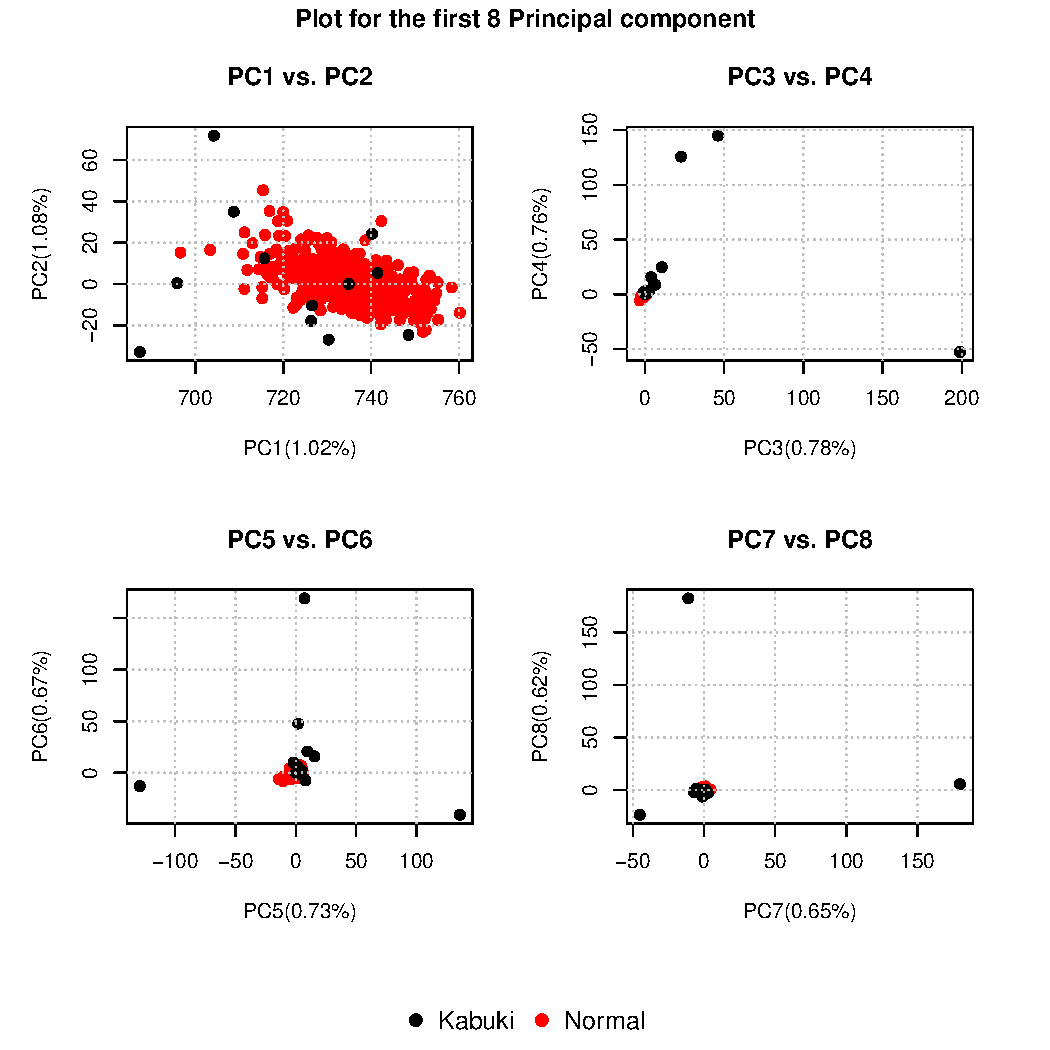
\includegraphics[width=\textwidth]{figures/PCA/1m/pca_plot.pdf}
    \caption{PCA plot for 1 million random features}
    \label{fig:1m-PCA}
\end{figure}

\begin{figure}[!h]
    \centering
    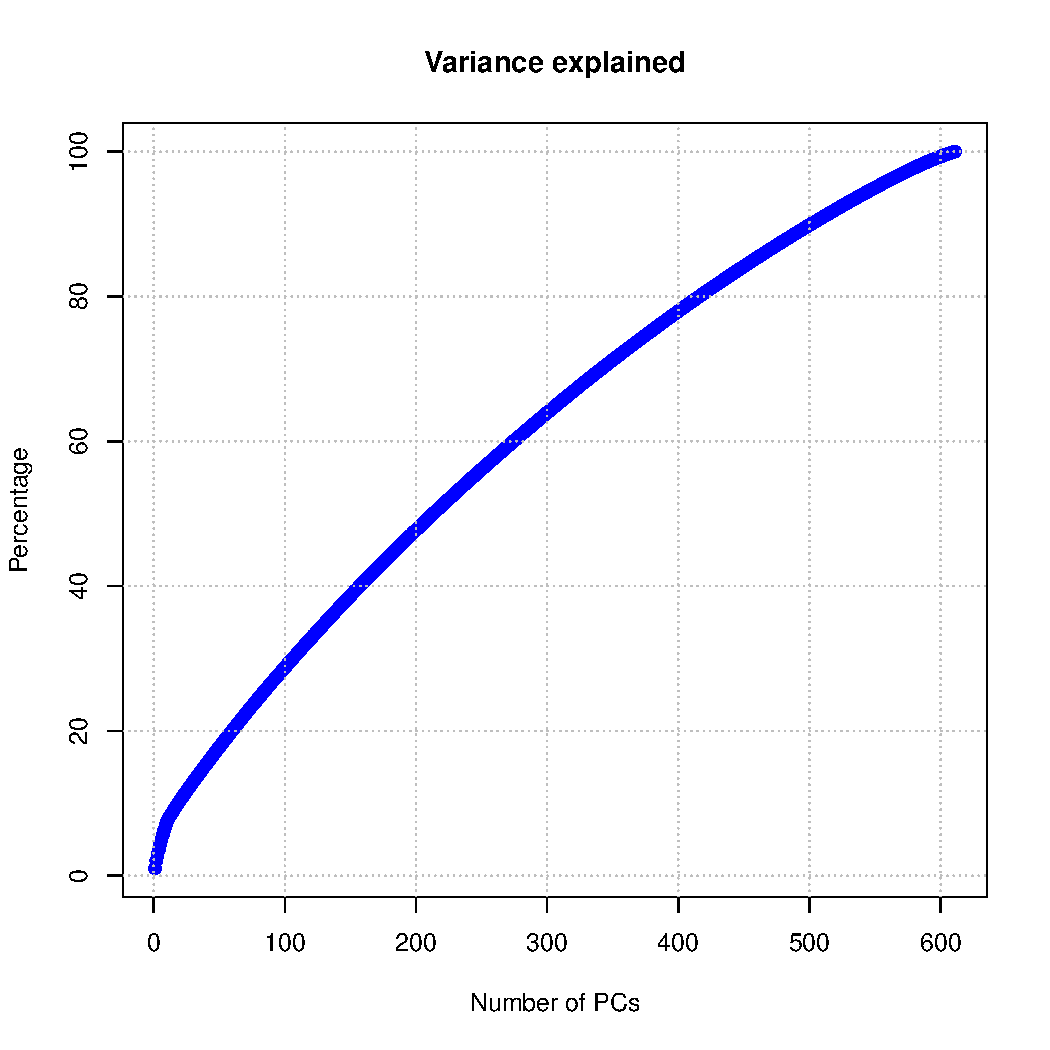
\includegraphics[width=0.5\columnwidth]{figures/PCA/1m/var_expl.pdf}
    \caption{Variance explained plot for 1 million random features}
    \label{fig:1m-varexpl}
\end{figure}
\FloatBarrier

\subsection{590 features}
In the first subplot in Figure \ref{fig:590-PCA} we can see that we can separate the groups using linear classifier, which indicates that those positions indeed are relevant for the Kabuki syndrome.

\begin{figure}[!h]
    \centering
    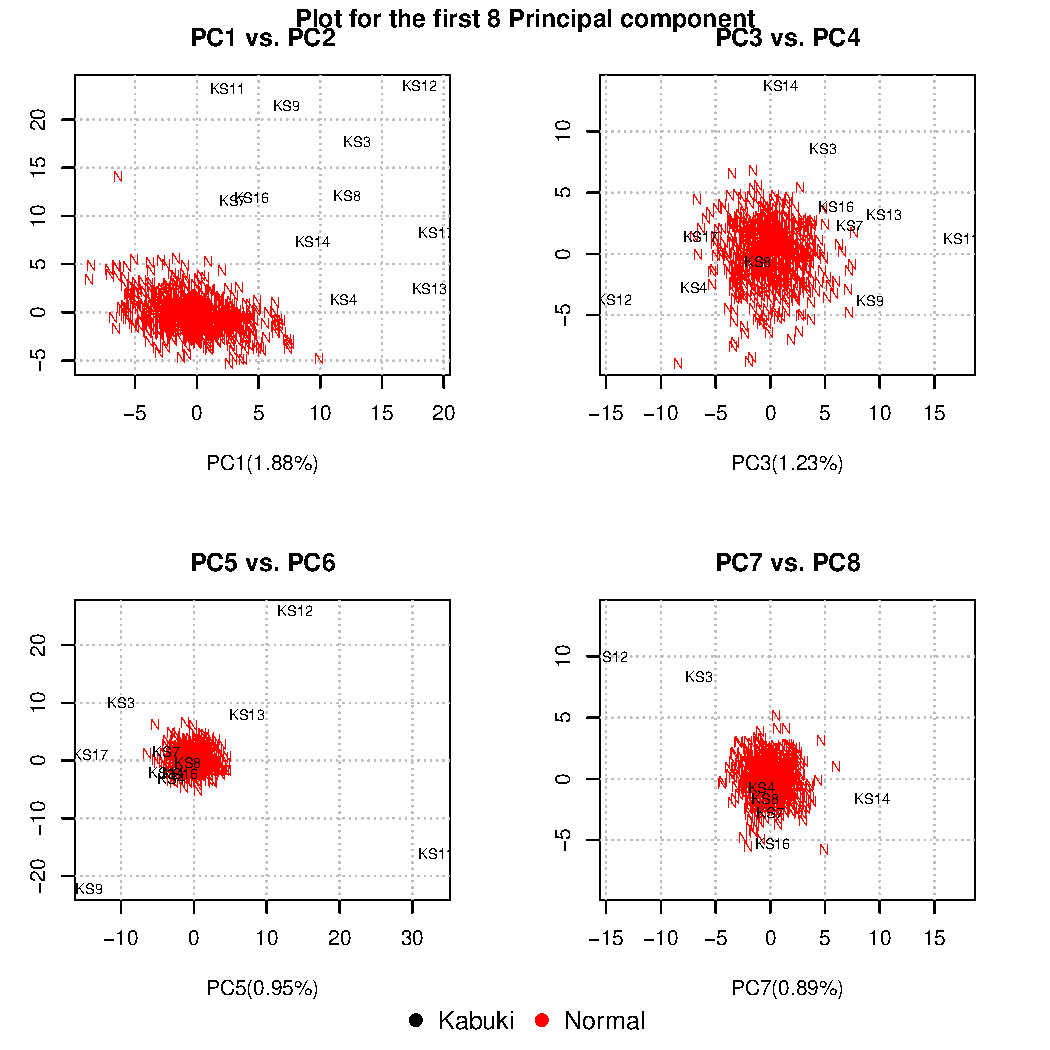
\includegraphics[width=\textwidth]{figures/PCA/590/pca_plot_label.pdf}
    \caption{PCA plot for 590 features known to be related to Kabuki syndrome}
    \label{fig:590-PCA}
\end{figure}
\begin{figure}[!h]
    \centering
    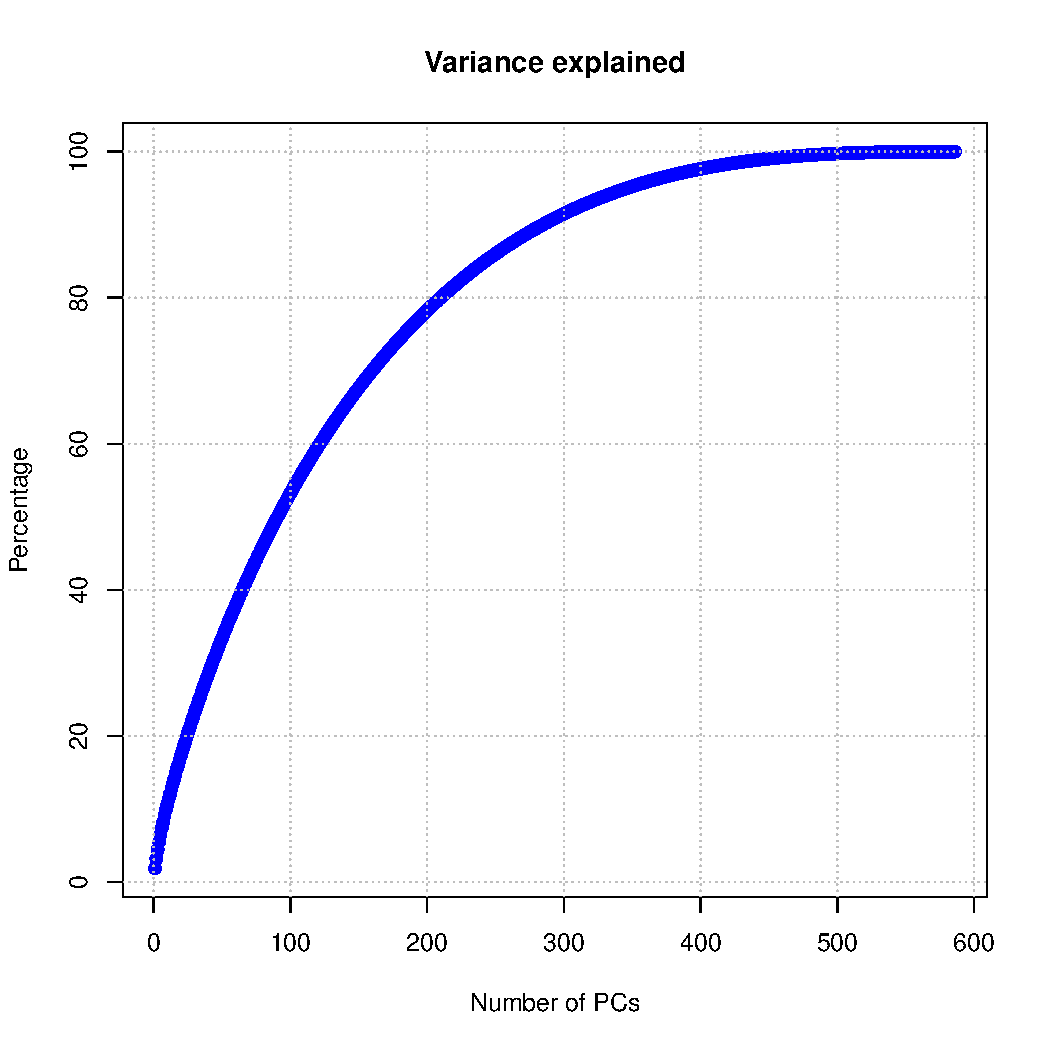
\includegraphics[width=0.5\columnwidth]{figures/PCA/590/var_expl.pdf}
    \caption{Variance explained plot for 590 features known to be related to Kabuki syndrome}
    \label{fig:590-varexpl}
\end{figure}
\

\subsection{Age matched dataset}
We performed PCA on all features (~22 million) of the age matched dataset. In Figure \ref{fig:case_control}-\ref{fig:case_control-sex} similarly as before we can see a lot more outliers in the Kabuki group. In the third subplot (PC5 vs PC6) we can almost perfectly separate the two groups using vertical line, however the other plots do not show decisive clustering.
\
\begin{figure}[!h]
    \centering
    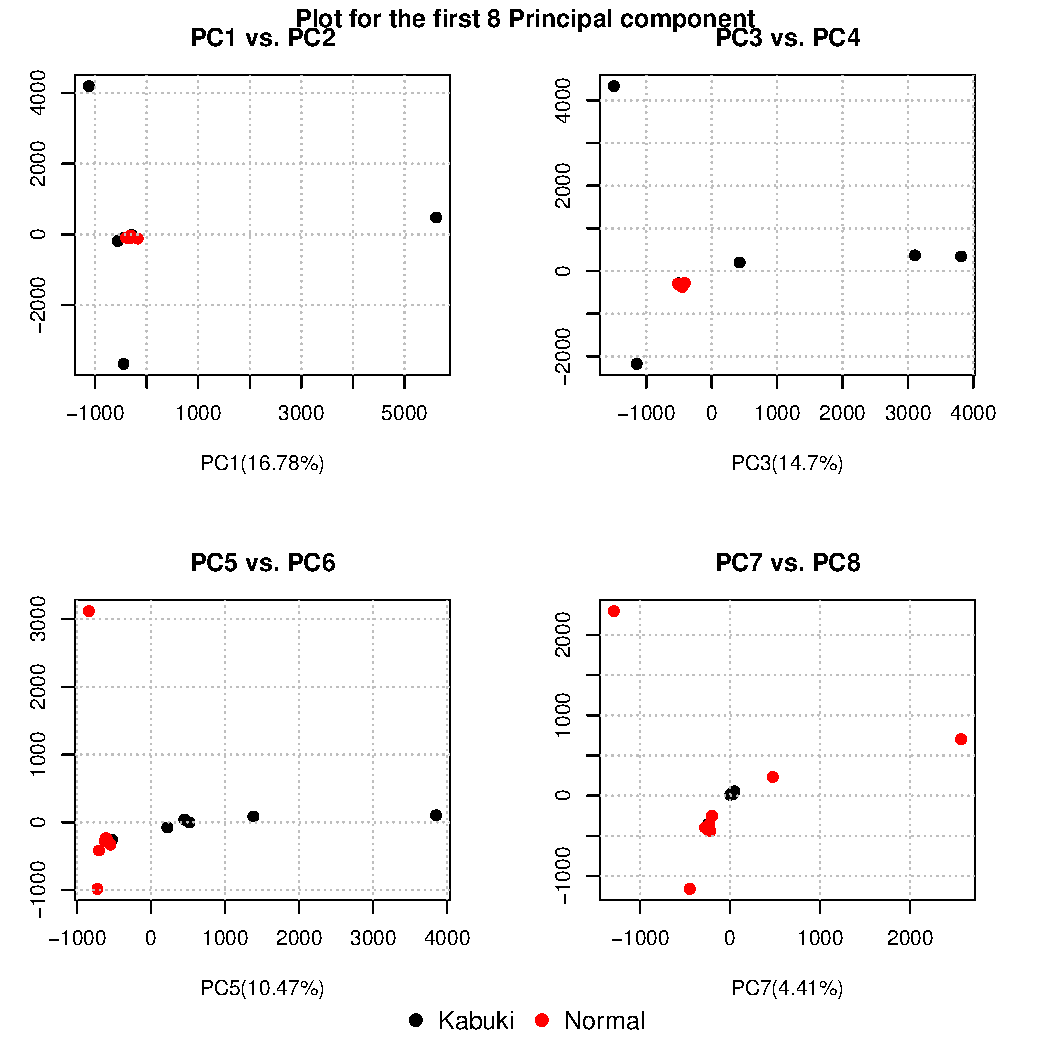
\includegraphics[width=\textwidth]{figures/PCA/case_control/pca_plot.pdf}
    \caption{PCA for the age matched dataset}
    \label{fig:case_control}
\end{figure}

\begin{figure}[!h]
    \centering
    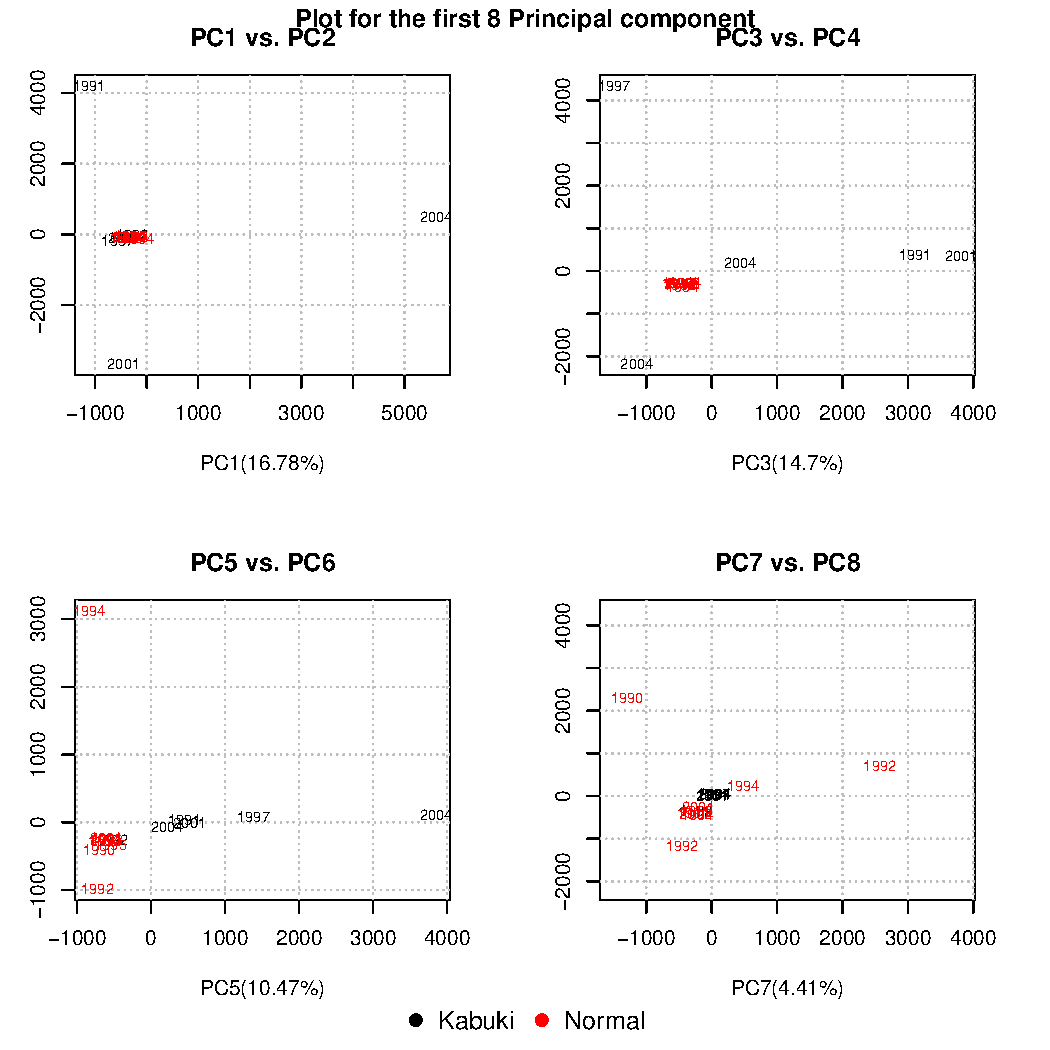
\includegraphics[width=\textwidth]{figures/PCA/case_control/age_PCA.pdf}
    \caption{PCA for the age matched dataset, with birth year displayed on the graph}
    \label{fig:case_control-age}
\end{figure}

\begin{figure}[!h]
    \centering
    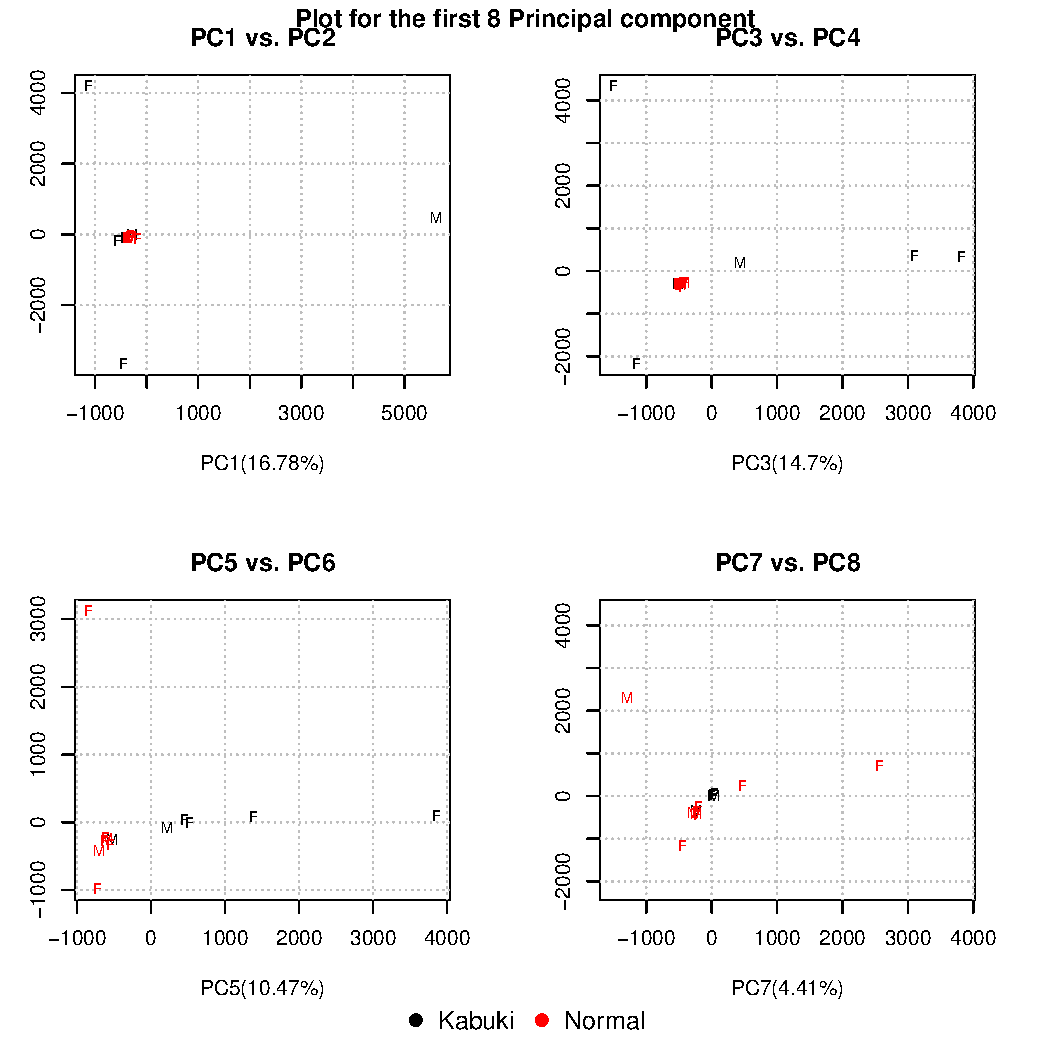
\includegraphics[width=\textwidth]{figures/PCA/case_control/sex_PCA.pdf}
    \caption{PCA for the age matched dataset, with sex displayed on the graph}
    \label{fig:case_control-sex}
\end{figure}




\subsection{Kabuki divided in two age groups}
We performed PCA on all features (~22 million) in the dataset. In Figure \ref{fig:oldyoung-pca} we have no clear clustering.
\begin{figure}[!h]
    \centering
    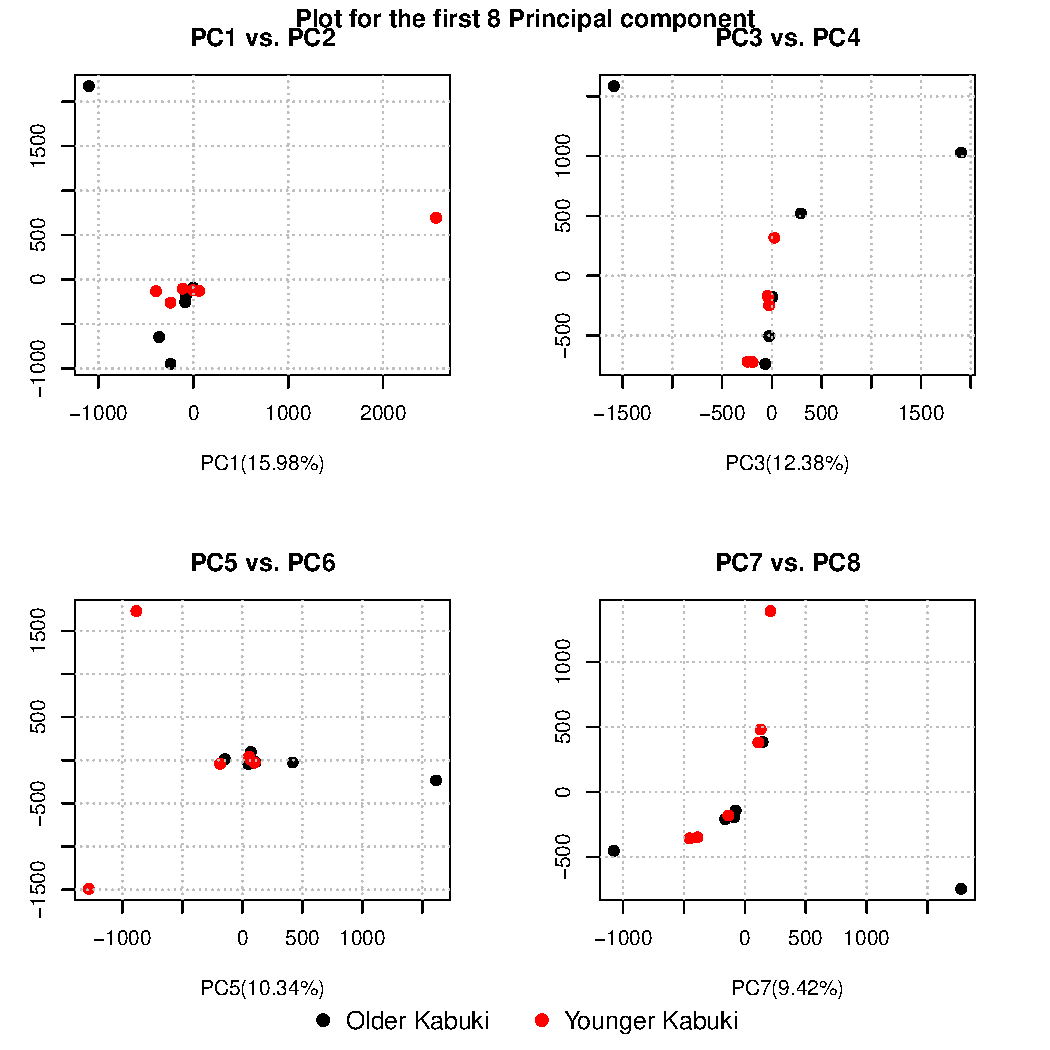
\includegraphics[width=\textwidth]{figures/PCA/old_young/pca_plot.pdf}
    \caption{PCA for the age divided kabuki dataset}
    \label{fig:oldyoung-pca}
\end{figure}
%%%%%%%%%%%%%%%%%%%%%%%%%%%%%%%%%%%%%%%%%%%%%%%%%%%%%%%%%%%%%%%%%%%%%%%%%%%%%%%%%%%
\iffalse
\begin{figure}[!h]
    \centering
    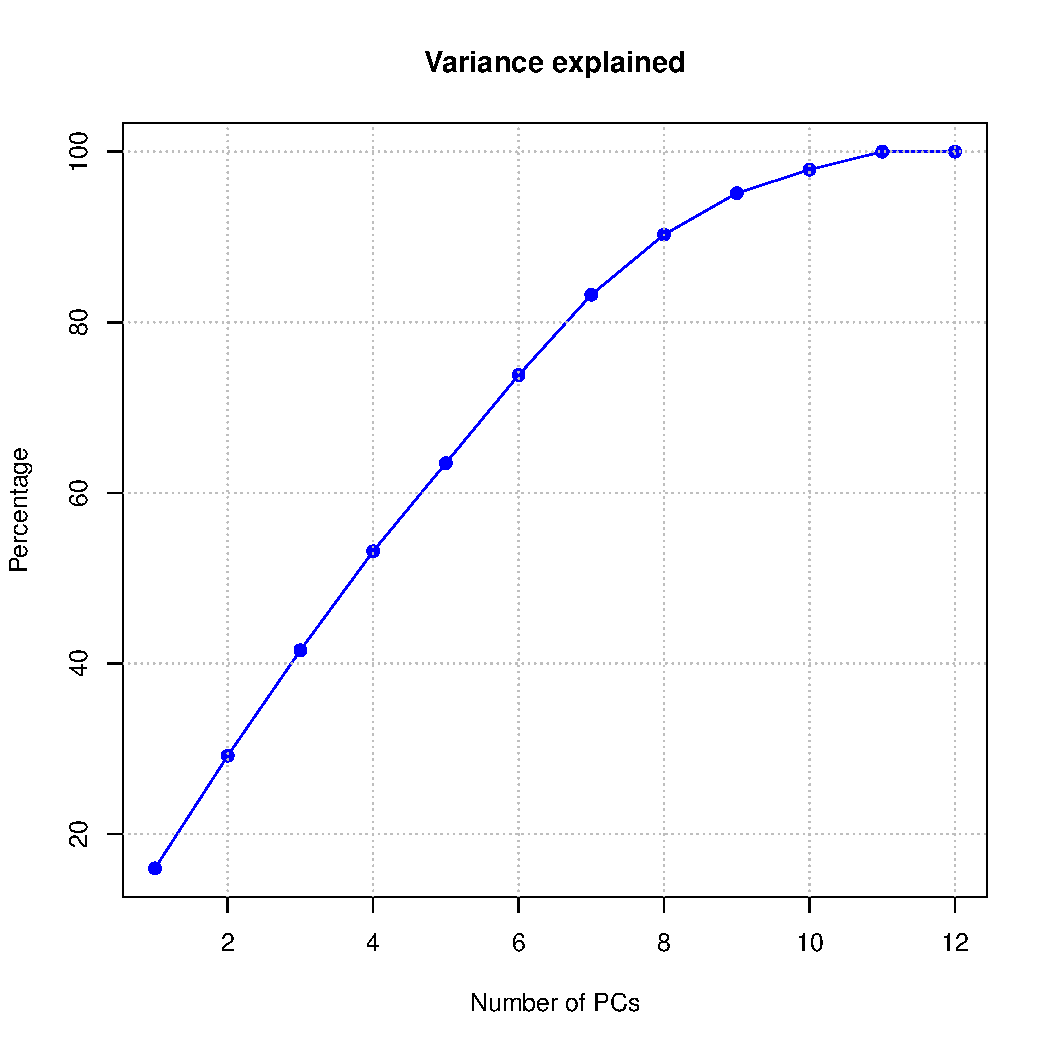
\includegraphics[width=0.6\columnwidth]{figures/PCA/old_young/var_expl.pdf}
    \caption{Variance explained for the age divided kabuki dataset}
    \label{fig:oldyoung-varexpl}
\end{figure}
\fi
%%%%%%%%%%%%%%%%%%%%%%%%%%%%%%%%%%%%%%%%%%%%%%%%%%%%%%%%%%%%%%%%%%%%%%%%%%%%%%%%%%


\subsection{Called with certainty}

\begin{figure}[!h]
    \centering
    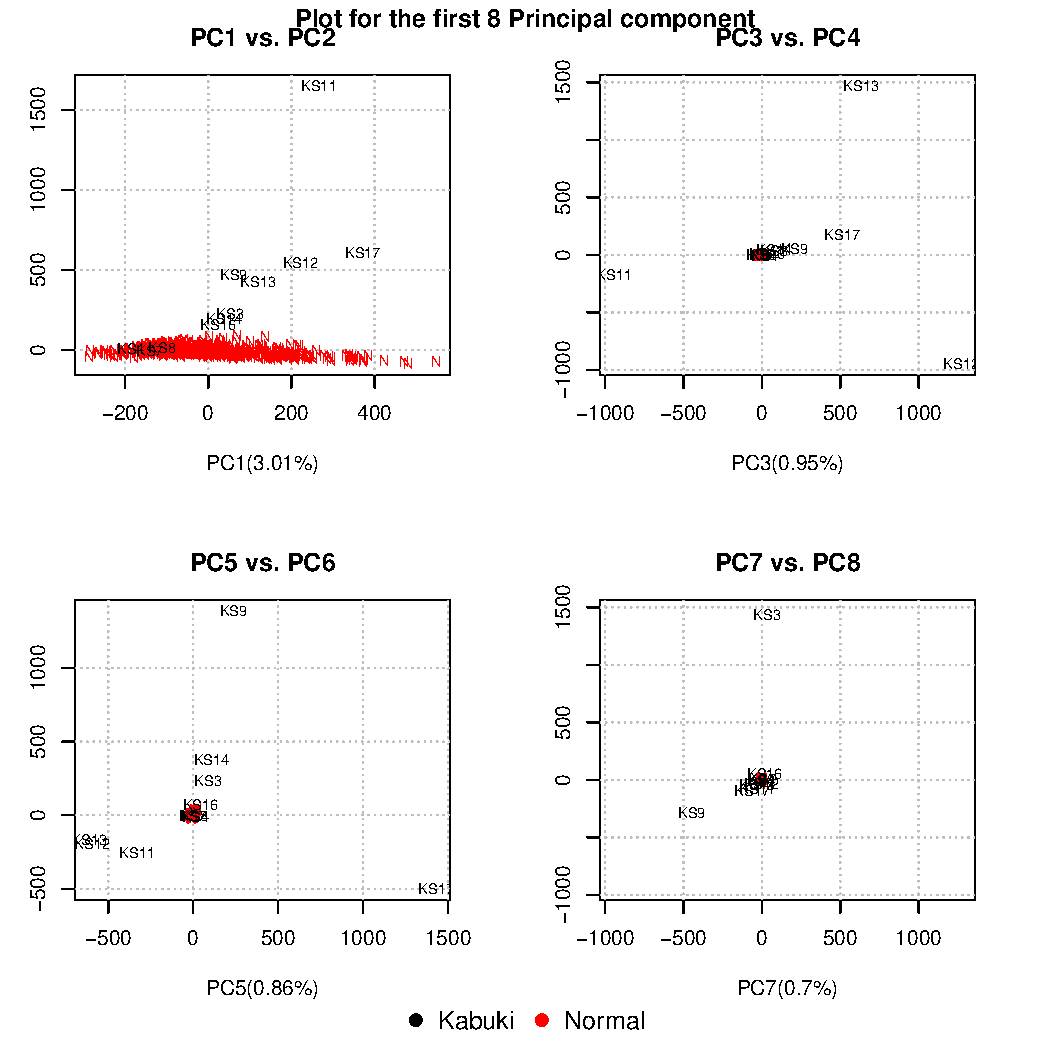
\includegraphics[width=\textwidth]{figures/PCA/certain/pca_plot_label.pdf}
    \caption{PCA plot for the features where nanopolish called methylation or non-methylation in over 90\% of the reads}
    \label{fig:certain-PCA}
\end{figure}

%%%%%%%%%%%%%%%%%%%%%%%%%%%%%%%%%%%%%%%%%%%%%%%%%%%%%%%%%%%%%%%%%%%%%%%%%%%%%%%%%%%
\iffalse
\begin{figure}[!h]
    \centering
    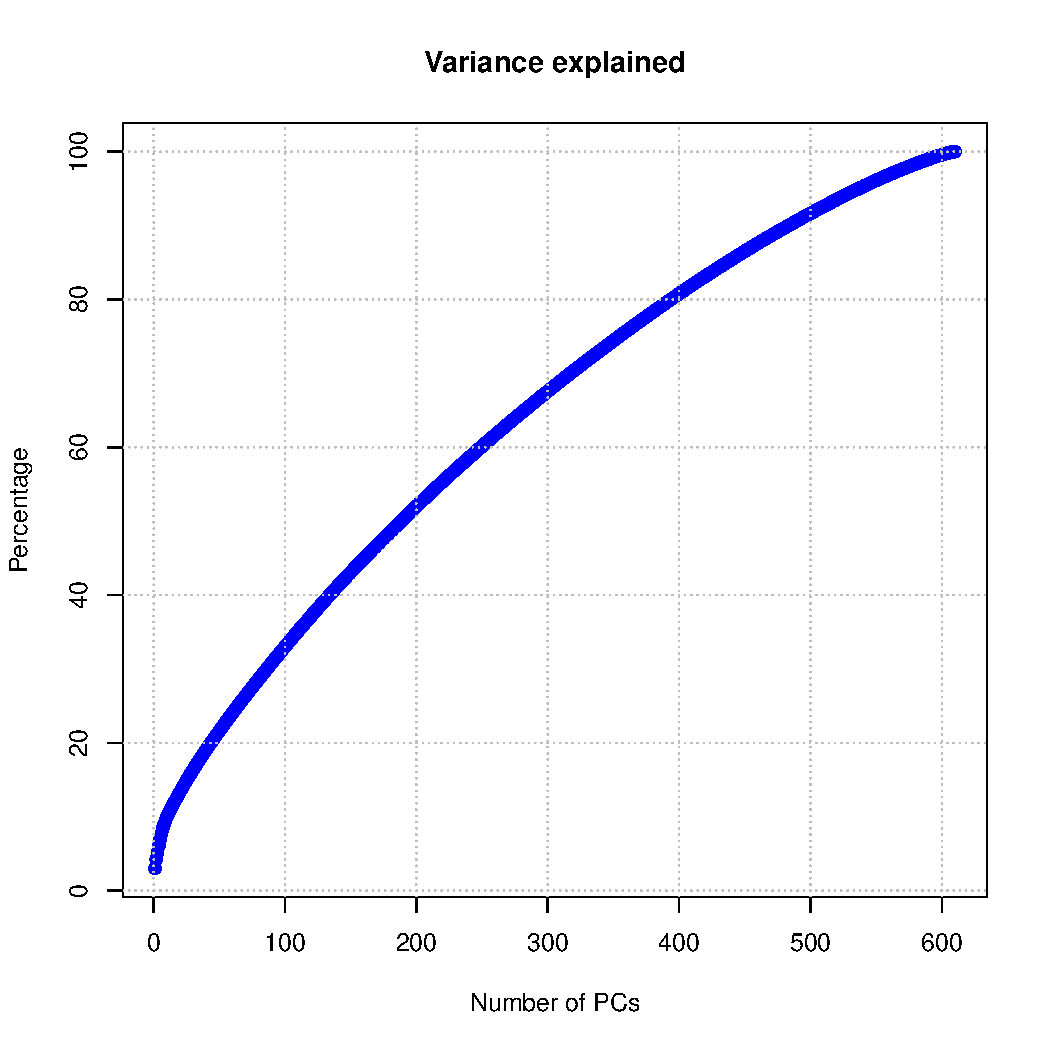
\includegraphics[width=0.6\columnwidth]{figures/PCA/certain/var_expl.pdf}
    \caption{Variance explained plot for the features where nanopolish called methylation or non-methylation in over 90\% of the reads}
    \label{fig:certain-varexpl}
\end{figure}
\fi
%%%%%%%%%%%%%%%%%%%%%%%%%%%%%%%%%%%%%%%%%%%%%%%%%%%%%%%%%%%%%%%%%%%%%%%%%%%%%%%%%%

\subsubsection{Bivalent regions}
\begin{figure}[!h]
    \centering
    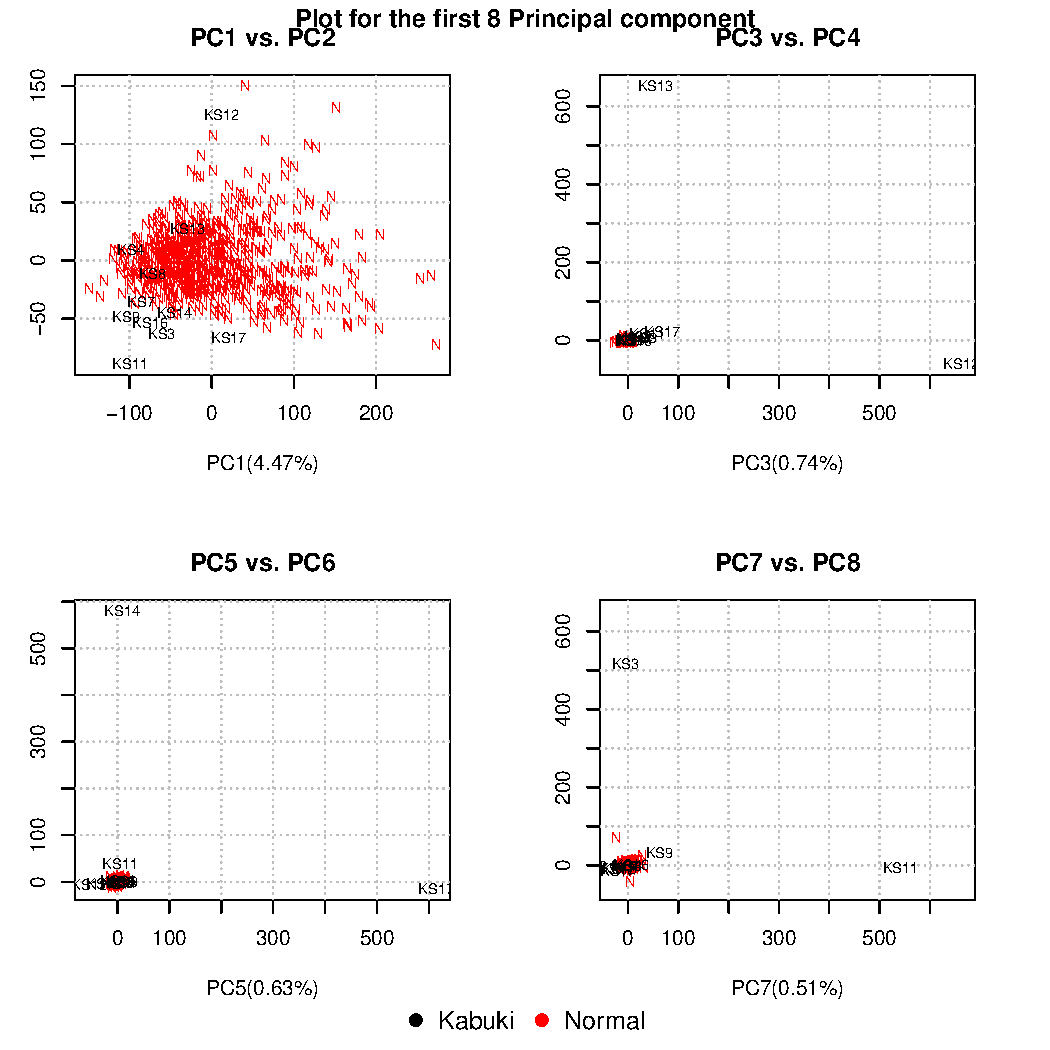
\includegraphics[width=\textwidth]{figures/PCA/bivalent/pca_plot_label.pdf}
    \caption{PCA plot for the features where nanopolish called methylation or non-methylation in over 90\% of the reads, within bivalent regions}
    \label{fig:bivalent-PCA}
\end{figure}

%%%%%%%%%%%%%%%%%%%%%%%%%%%%%%%%%%%%%%%%%%%%%%%%%%%%%%%%%%%%%%%%%%%%%%%%%%%%%%%%%%%
\iffalse
\begin{figure}[!h]
    \centering
    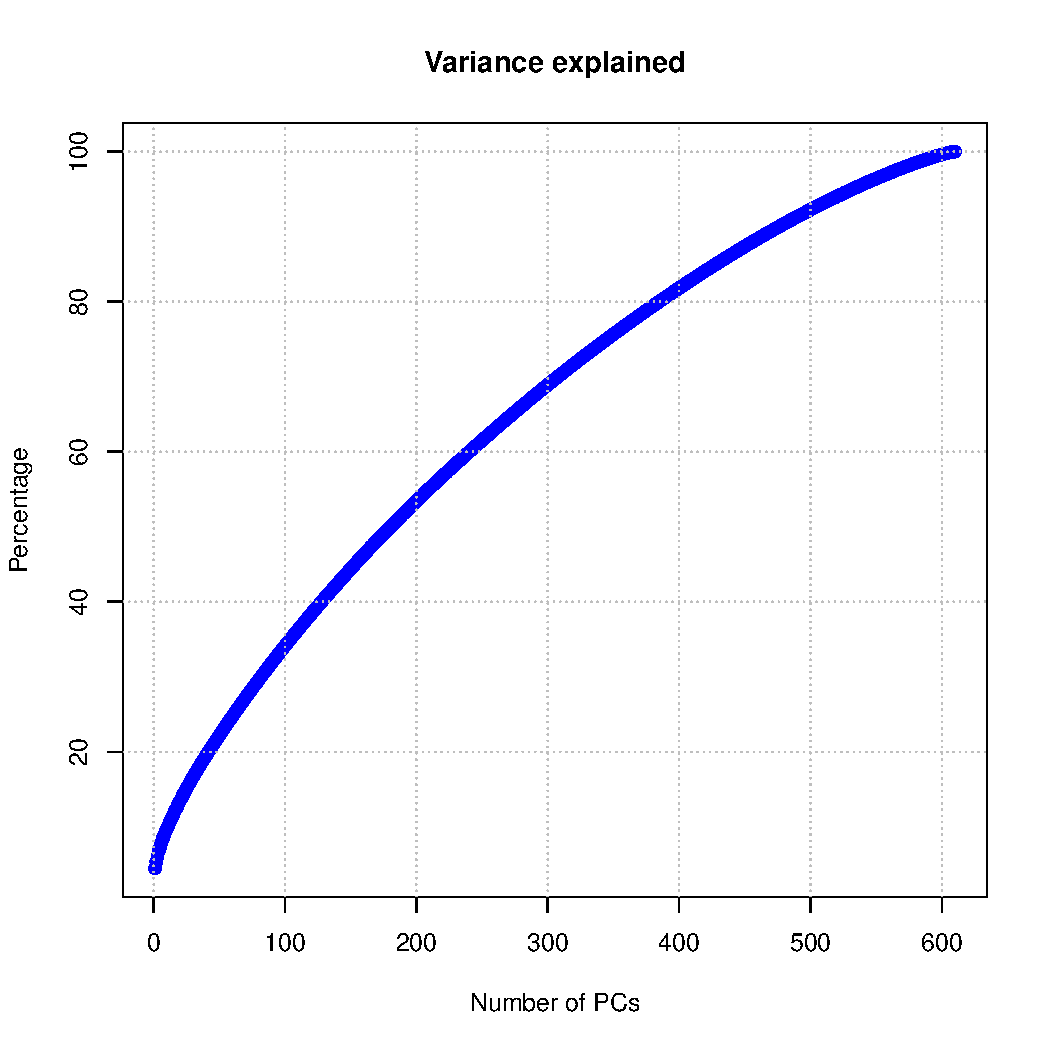
\includegraphics[width=0.6\columnwidth]{figures/PCA/bivalent/var_expl.pdf}
    \caption{Variance explained plot for the features where nanopolish called methylation or non-methylation in over 90\% of the reads, within bivalent regions}
    \label{fig:bivalent-varexpl}
\end{figure}
\fi
%%%%%%%%%%%%%%%%%%%%%%%%%%%%%%%%%%%%%%%%%%%%%%%%%%%%%%%%%%%%%%%%%%%%%%%%%%%%%%%%

\subsection{Consistency between plus and minus strand}

\begin{figure}[!h]
    \centering
    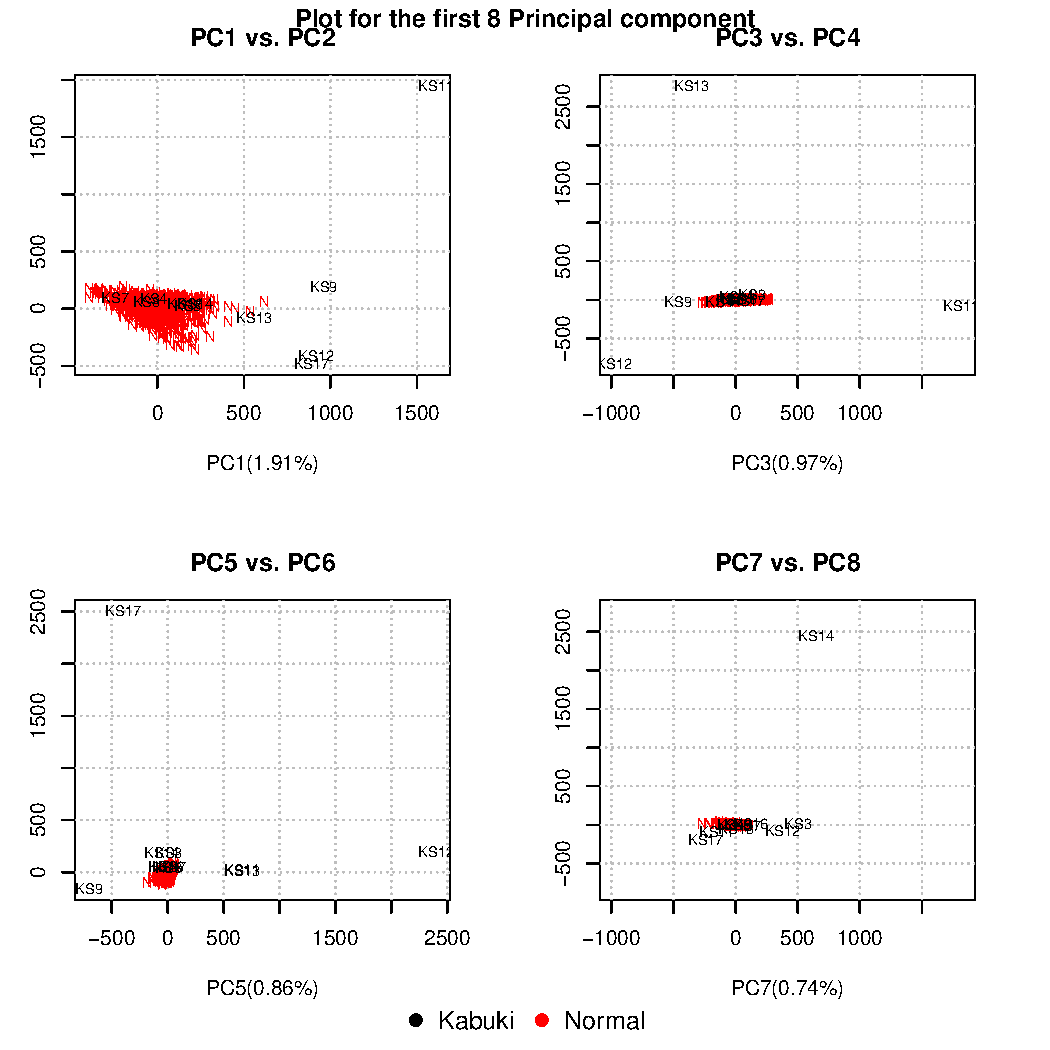
\includegraphics[width=\textwidth]{figures/PCA/plus_minus/pca_plot_label.pdf}
    \caption{PCA plot for the features where nanopolish had less than 0.5\% difference between the plus strand and minus strand}
    \label{fig:certain-PCA}
\end{figure}

%%%%%%%%%%%%%%%%%%%%%%%%%%%%%%%%%%%%%%%%%%%%%%%%%%%%%%%%%%%%%%%%%%%%%%%%%%%%%%%%%%%
\iffalse
\begin{figure}[!h]
    \centering
    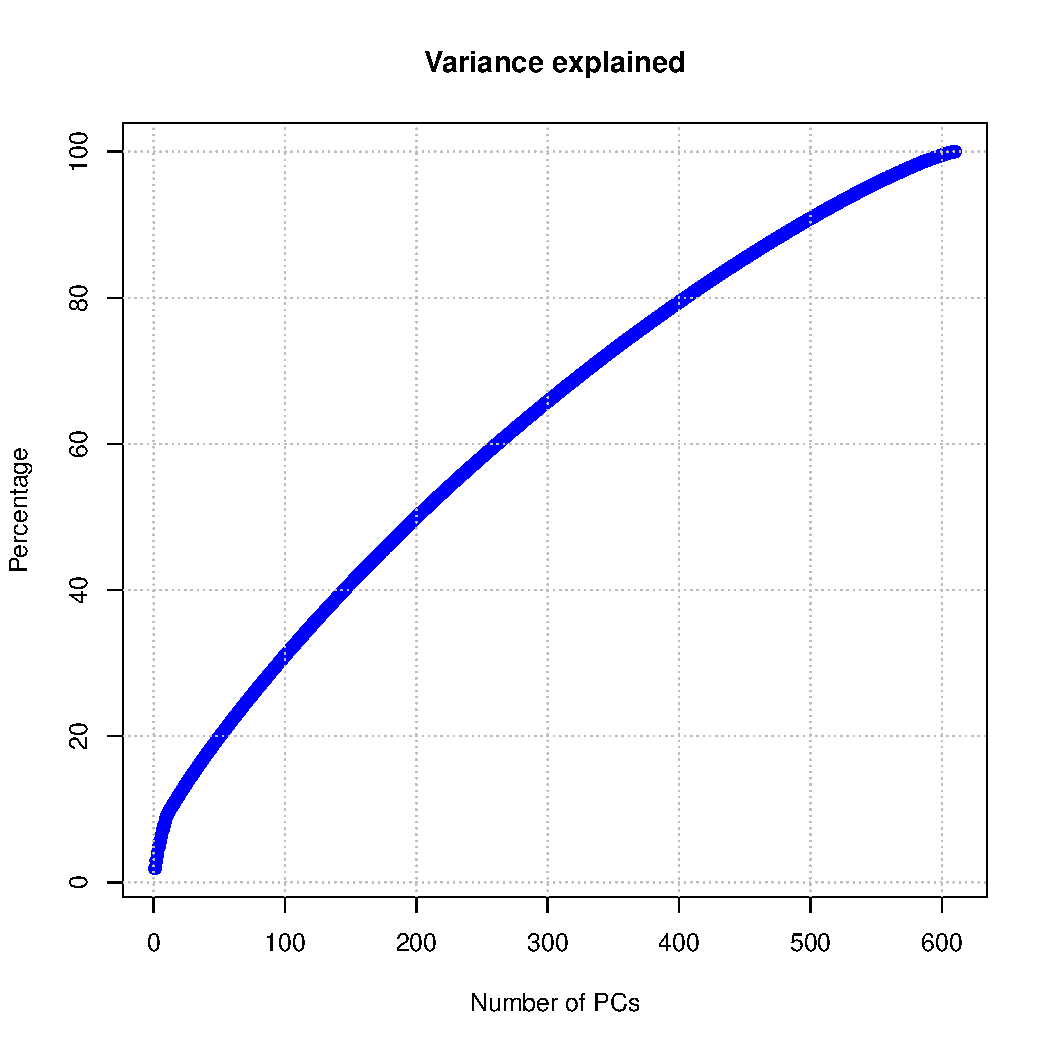
\includegraphics[width=0.6\columnwidth]{figures/PCA/plus_minus/var_expl.pdf}
    \caption{Variance explained plot for the features where nanopolish had less than 0.5\% difference between the plus strand and minus strand}
    \label{fig:certain-varexpl}
\end{figure}
\fi
%%%%%%%%%%%%%%%%%%%%%%%%%%%%%%%%%%%%%%%%%%%%%%%%%%%%%%%%%%%%%%%%%%%%%%%%%%%%%%%%%

\subsection{590 larger}
\iffalse
\begin{figure}[!h]
    \centering
    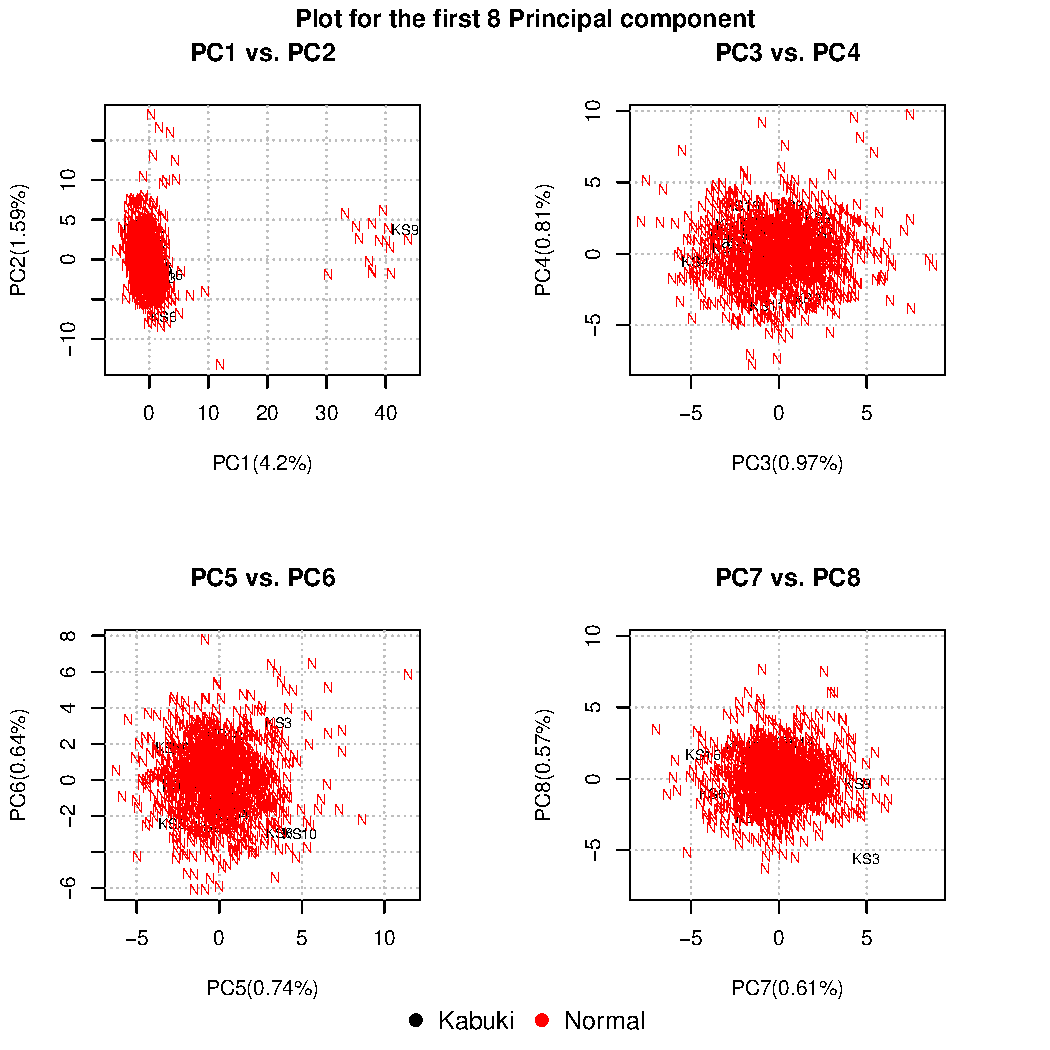
\includegraphics[width=\textwidth]{figures/PCA/590/pca_plot_label_larger.pdf}
    \caption{PCA plot for the final dataset, for the 590 positions identified by H.Tomasson.}
    \label{fig:certain-PCA}
\end{figure}

\subsection{Certain larger}

\begin{figure}[!h]
    \centering
    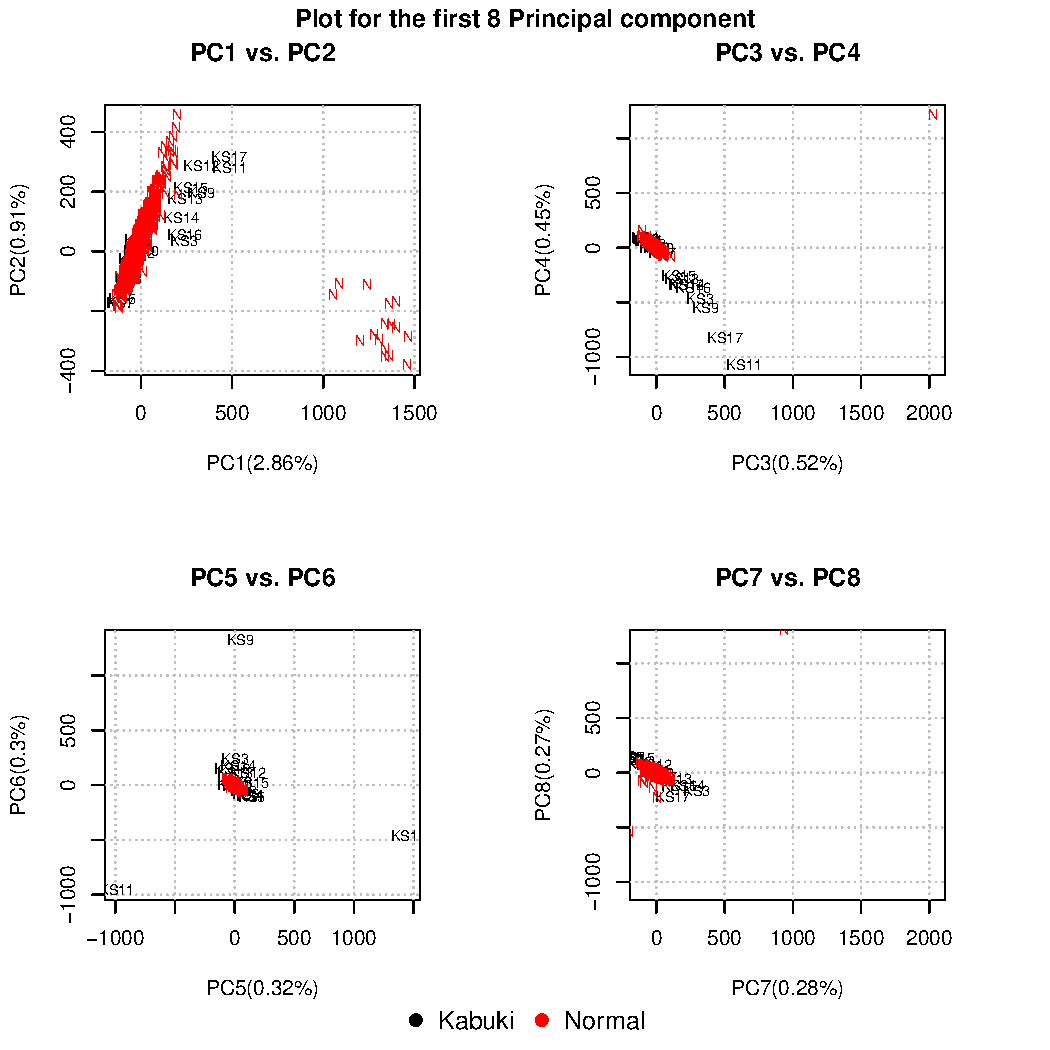
\includegraphics[width=\textwidth]{figures/PCA/certain/pca_plot_label_larger.pdf}
    \caption{PCA plot for the final dataset, where methylation or non-methylation was called in >75\% of the reads..}
    \label{fig:certain-PCA}
\end{figure}
\fi 

\subsection{Bonferroni}
\begin{figure}[!h]
    \centering
    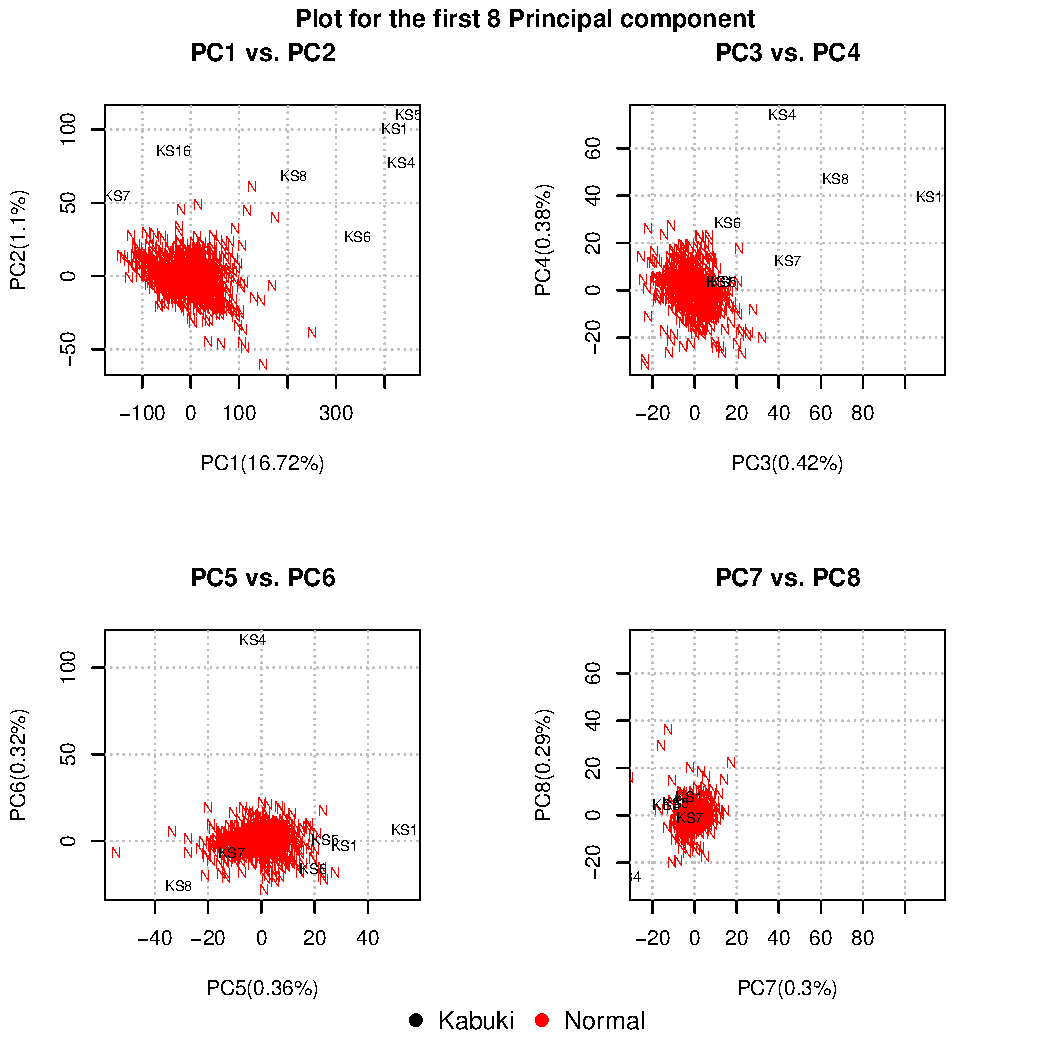
\includegraphics[width=\textwidth]{figures/PCA/bonferroni/pca_plot_label.pdf}
    \caption{PCA plot are considered significantly differentially methylated given the bonferroni threshold}
    \label{fig:bonferroni-PCA}
\end{figure}


\section{Hierarchical clustering}
We performed Hierarchical clustering using dist() and hclust() in R \ref{fig:hclust}. It can be seen that most of the Kabuki samples form a cluster, however there are three kabuki samples distributed within the control group.

\begin{figure}[!h]
    \begin{centering}
    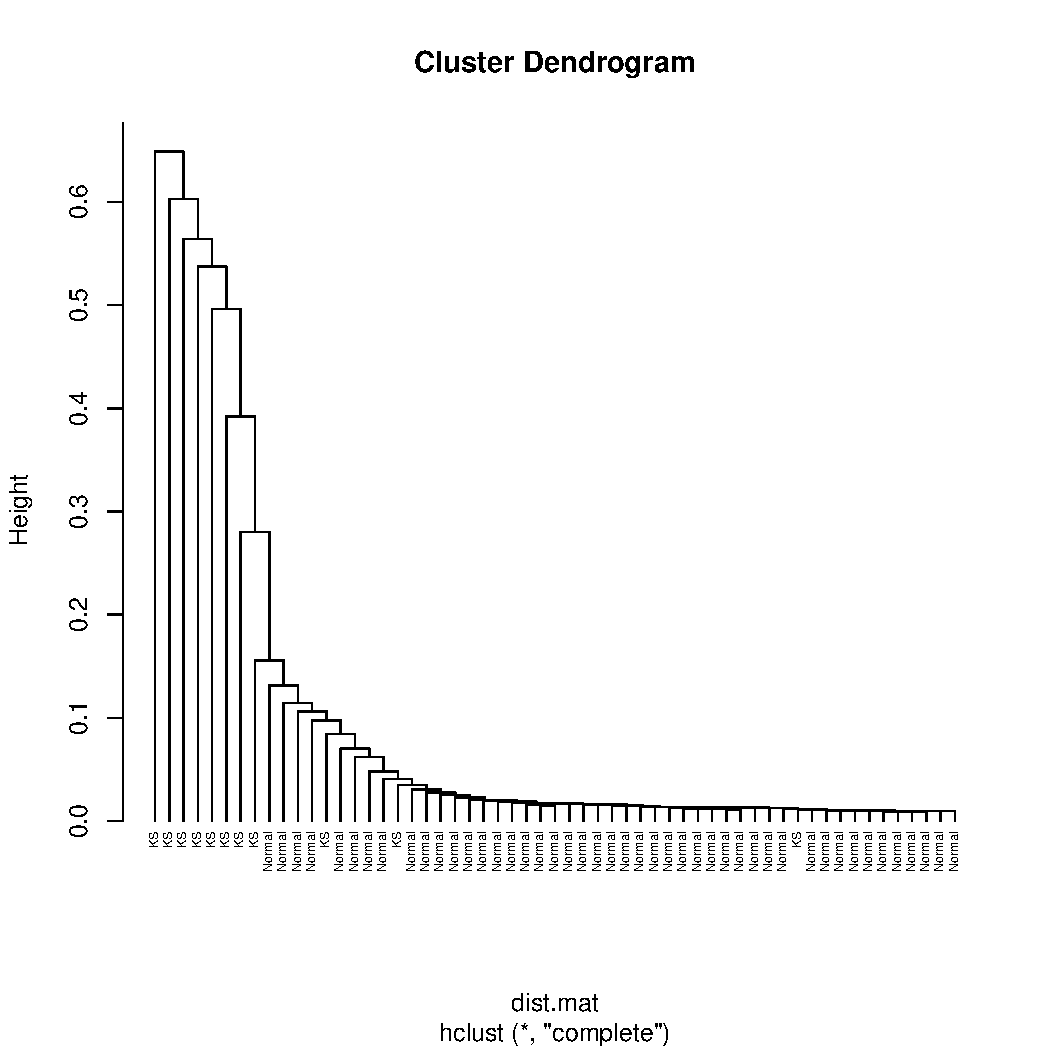
\includegraphics[width=0.7\columnwidth]{figures/hclust.pdf} 
    \caption[Hierachical clustering]{\textbf{Hierarchical clustering.} Clustering bla bla bla}    
    \label{fig:hclust}
    \end{centering}
\end{figure}

% Also insert from the 590

\section{Average methylation per grop}

\begin{figure}[!h]
    \begin{centering}
    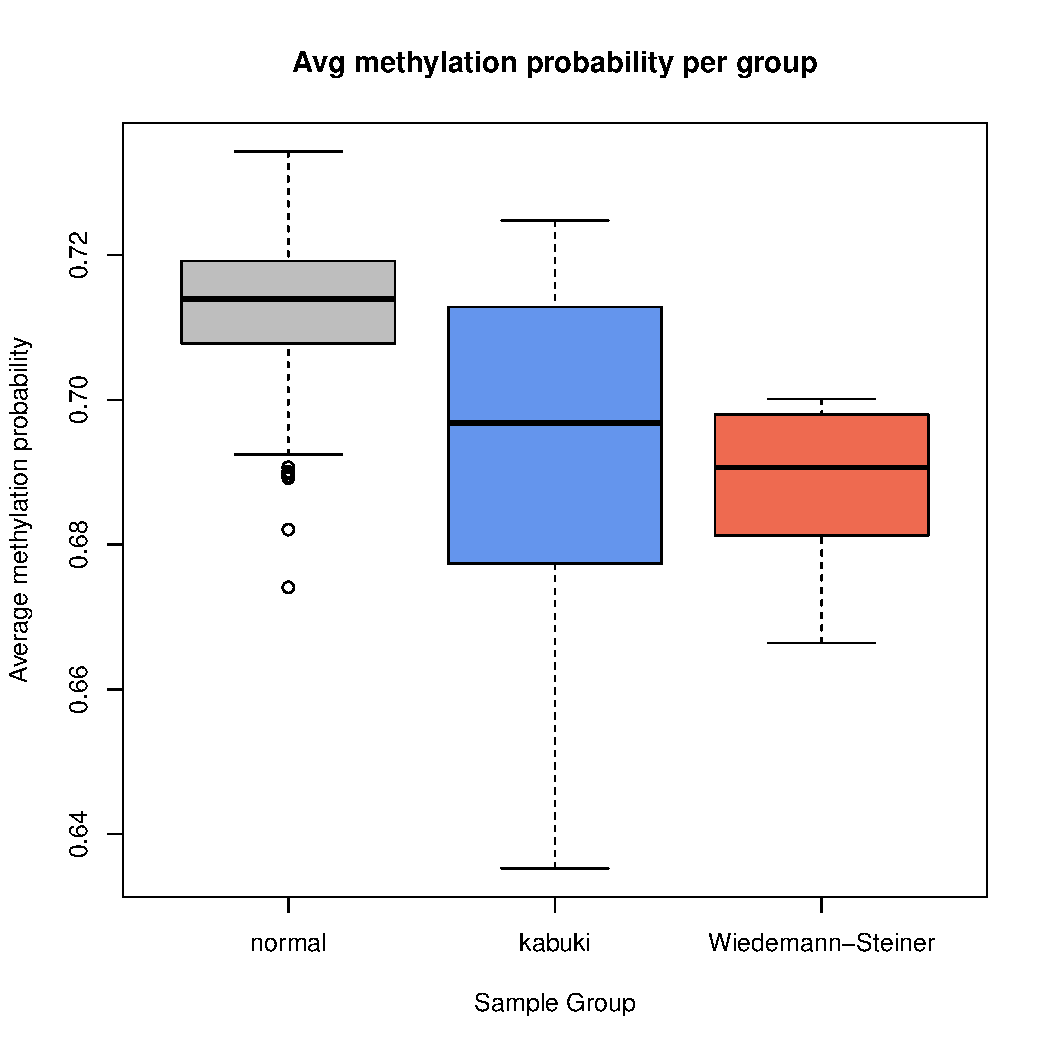
\includegraphics[width=0.7\columnwidth]{figures/avg_met_per_group.pdf} 
    \caption[Average methylation per sample group]{\textbf{Average methylation per group.} We can see that the average methylation for the normal group is a little bit higher then for the other two. However we also have more samples and therefore the measurement is also more accurate.}    
    \label{fig:hclust}
    \end{centering}
\end{figure}

\section{Nanopolish performance}
\label{section:results:Nanopolish-performance}
We took the Nanopolish results for 9 individuals from the control group and used for the performance estimate of Nanopolish. First we calculated the average methylation ratio per position over the subset. Next we calculated the average methylation ratio reported within methylation regions and unmethylated regions. Those calculations we did both using the original nanopolish model as well as the retrained model. The results are shown in Table \ref{table:nanopolish-performance1}.

\begin {table}
    \caption{Average methylation calling for each region type}
    \begin{center}
        \begin{tabular}{l l l } 
            \hline
             \textbf{Methylation status} & \textbf{Old model} & \textbf{New model}\\
             \hline
             \hline
              \multicolumn{3}{c}{Methylated regions} \\
             \hline
             \textbf{Methylated} & 0.646543 & 0.667892 \\ 
             \textbf{Unknown} & 0.304928 & 0.283442\\
             \textbf{Unmethylated} & 0.0485266 & 0.0486634\\ 
             \hline
            \multicolumn{3}{c}{Unmethylated region} \\
            \hline
             \textbf{Methylated} & 0.289242 & 0.263843 \\ 
             \textbf{Unknown} & 0.272034 & 0.235587\\
             \textbf{Unmethylated} & 0.438722 & 0.500568\\ 
             \hline
        \end{tabular}
    \label{table:nanopolish-performance1}
    \end{center}
\end{table}

We removed reads where we interprate the methylation status as unknown and recalculated the percentages for each region type. Results are shown in Table \ref{table:nanopolish-performance2}.

\begin {table}
    \caption{Average methylation ratio for each region type, after removing reads with unknown methylation status}
    \begin{center}
        \begin{tabular}{c c c } 
            \hline
            \textbf{Methylation status} & \textbf{Old model} & \textbf{New model}\\
             \hline
             \hline
             \textbf{Methylated} & 0.924607 & 0.926313 \\ 
             \textbf{Unmethylated} & 0.416935 & 0.370074 \\ 
             \hline
        \end{tabular}
    \label{table:nanopolish-performance2}
    \end{center}
\end{table}



For the methylated regions we got the following results:
\begin{equation*}
    \begin{cases}
    MN = 0.639638 \\
    XN = 0.310874 \\ 
    UN = 0.0494866 \\ 
    \end{cases}
\end{equation*}

Which means that out of the reads where nanopolish is certain, it calls methylation in 92.8\% of the cases and non-methylated in 7.2\%. 

And for the unmethylated regions:
\begin{equation*}
    \begin{cases}
    MN=0.287836 \\
    XN=0.278107\\
    UN=0.434055\\ 
    \end{cases}
\end{equation*}

Meaning that out of the reads where nanopolish is certain, it calls methylation in 39.9\% of the cases and in 60.1\% of the cases it calls non-methylation.

Since the nanopolish model is trained on non-human, minION data and we use human, promethION data for our analysis we expected those numbers to improve if we retrained the model on our human promethION data. 


\subsection{Filtering}

\begin {table}
    \caption{Number of features selected for each filter}
    \begin{center}
        \begin{tabular}{ c c } 
            \hline
            \textbf{Filtering} & \textbf{Number of positions}\\
             \hline
             \hline
             \textbf{Plus/Minus strand} & 1,524,993  \\ 
             \textbf{Certainty} & 3,651,209 \\
             \hline
        \end{tabular}
    \label{table:cont}
    \end{center}
\end{table}

%We found that the average methylation probability over all regions that were known to be greater than 95\% or less then 20\% was 81.2\% and 43.5\%, respectively. These result indicate that nanopolish is not performing as well as expected. Since the nanopolish model was trained using MinION data we retrained the model using PromethION data.


After filtering out positions where nanopolish calls methylation or non-methylation in less than 80\% of the cases, nanopolish calls methylation in 23.31\% of the cases in the unmethylated region and non-methylation in 76.69\% of the cases. For the methylated region, nanopolish calls methylation in 95.65\% of the cases and non-methylation in 4.35\% of the cases.


\section{PRS}
lasso regression + upsampling/downsampling
%%%%%%%%%%%%%%%%%%%%%%%%%%%%%%%%%%%%%%%%%%%%%%%%%%%
%%%%%%%%%% COMMENTED OUT %%%%%%%%%%%%%%%%%%%%%%%%%%
%%%%%%%%%%%%%%%%%%%%%%%%%%%%%%%%%%%%%%%%%%%%%%%%%%%

\iffalse
\begin{figure}[!h]
     \centering
     \begin{subfigure}[b]{0.45\textwidth}
         \centering
         \includegraphics[width=\textwidth]{figures/pca_12_reduced.pdf}
         \caption{First two PCs}
         \label{fig:pca_1m1}
     \end{subfigure}
     \hfill
     \begin{subfigure}[b]{0.45\textwidth}
         \centering
         \includegraphics[width=\textwidth]{figures/pca_34_reduced.pdf}
         \caption{Third and fourth PCs}
         \label{fig:pca_1m2}
     \end{subfigure}
     \hfill
     \begin{subfigure}[b]{0.45\textwidth}
         \centering
         \includegraphics[width=\textwidth]{figures/var_expl_reduced.pdf}
         \caption{Variance explained}
         \label{fig:pca_1m3}
     \end{subfigure}
        \caption[PCA plot for 1 million random features]{\textbf{PCA plot for 1 million random features.} We can see that the PCA clustering does not show a good clustering, we have three samples from the Kabuki group as outliers.}
        \label{fig:PCA_1m}
\end{figure}
\fi

%%%%%%%%%%%%%%%%%%%%%%%%%%%%%%%%%%%%%%%%%%%%%%%%%%%
%%%%%%%%%%%%%%%%%%%%%%%%%%%%%%%%%%%%%%%%%%%%%%%%%%%
%%%%%%%%%%%%%%%%%%%%%%%%%%%%%%%%%%%%%%%%%%%%%%%%%%%



\include{ltablex}




% This displays the bibliography for all cited external documents. All references have to be defined in the file references.bib and can then be cited from within this document.
\listoftables
\listoffigures
\bibliographystyle{IEEEtran}
\bibliography{references}

% This creates an appendix chapter, comment if not needed.
\appendix
\chapter{First Appendix Chapter Title}

\end{document}